\documentclass[aspectratio=169]{beamer}

\setbeamertemplate{footline}[frame number]

\usepackage{hyperref}
\usepackage{caption}
\captionsetup[figure]{labelformat=empty}

\title{Exploratory analysis of Recurrent deforestation warnings in the 
Brazilian Amazon}

\author{Alber Sanchez\\alber.ipia@inpe.br}
\institute{
    
\includegraphics[width=4cm,keepaspectratio]{./logos/trees-color-h_2.png}
    
\includegraphics[width=1.8cm,keepaspectratio]{./logos/logoinpe-azul-menor.png} \\
    TreesLab\\Instituto Nacional de Pesquisas Espaciais - INPE\\Brazil
}
\date{\today}

\begin{document}


%---- Introduction ----

\frame{\titlepage}

\begin{frame}
    \frametitle{Introduction}
    \begin{itemize}
        \item Deforestation by successive degradation remains a challenging 
            question in the scientific literature.
        \item We think an answer to this question lies down in DETER data.
        \item This answer could play an important role, for example, in the 
            brazilian estimation of greenhouse gases.
        \item We used DETER data from 2016 to 2021 of the Amazon Biome in 
              Brazil.
    \end{itemize}
\end{frame}



%---- DETER ----

\begin{frame}
    \frametitle{What is DETER?}
    \begin{itemize}
        \item DETER is a GIS which produces a fast assessment of deforestation 
            and forest degradation in the Brazilian 
            Amazon~\cite{shimabukuro2006}.
        \item DETER is an important tool for environmental protection and  
            effective law enforcement.
        \item DETER employs Linear Mixture Models of CBERS imagery and human
            experts to deter and issue warnings of deforested (or degraded) 
            areas larger than 3 ha~\cite{dealmeida2022}.
        \item Annually, DETER takes from PRODES the current forested area, 
            stating anew issuing warnings.
    \end{itemize}
\end{frame}

\begin{frame}
    \frametitle{DETER warnings}
    \begin{figure}[h] 
        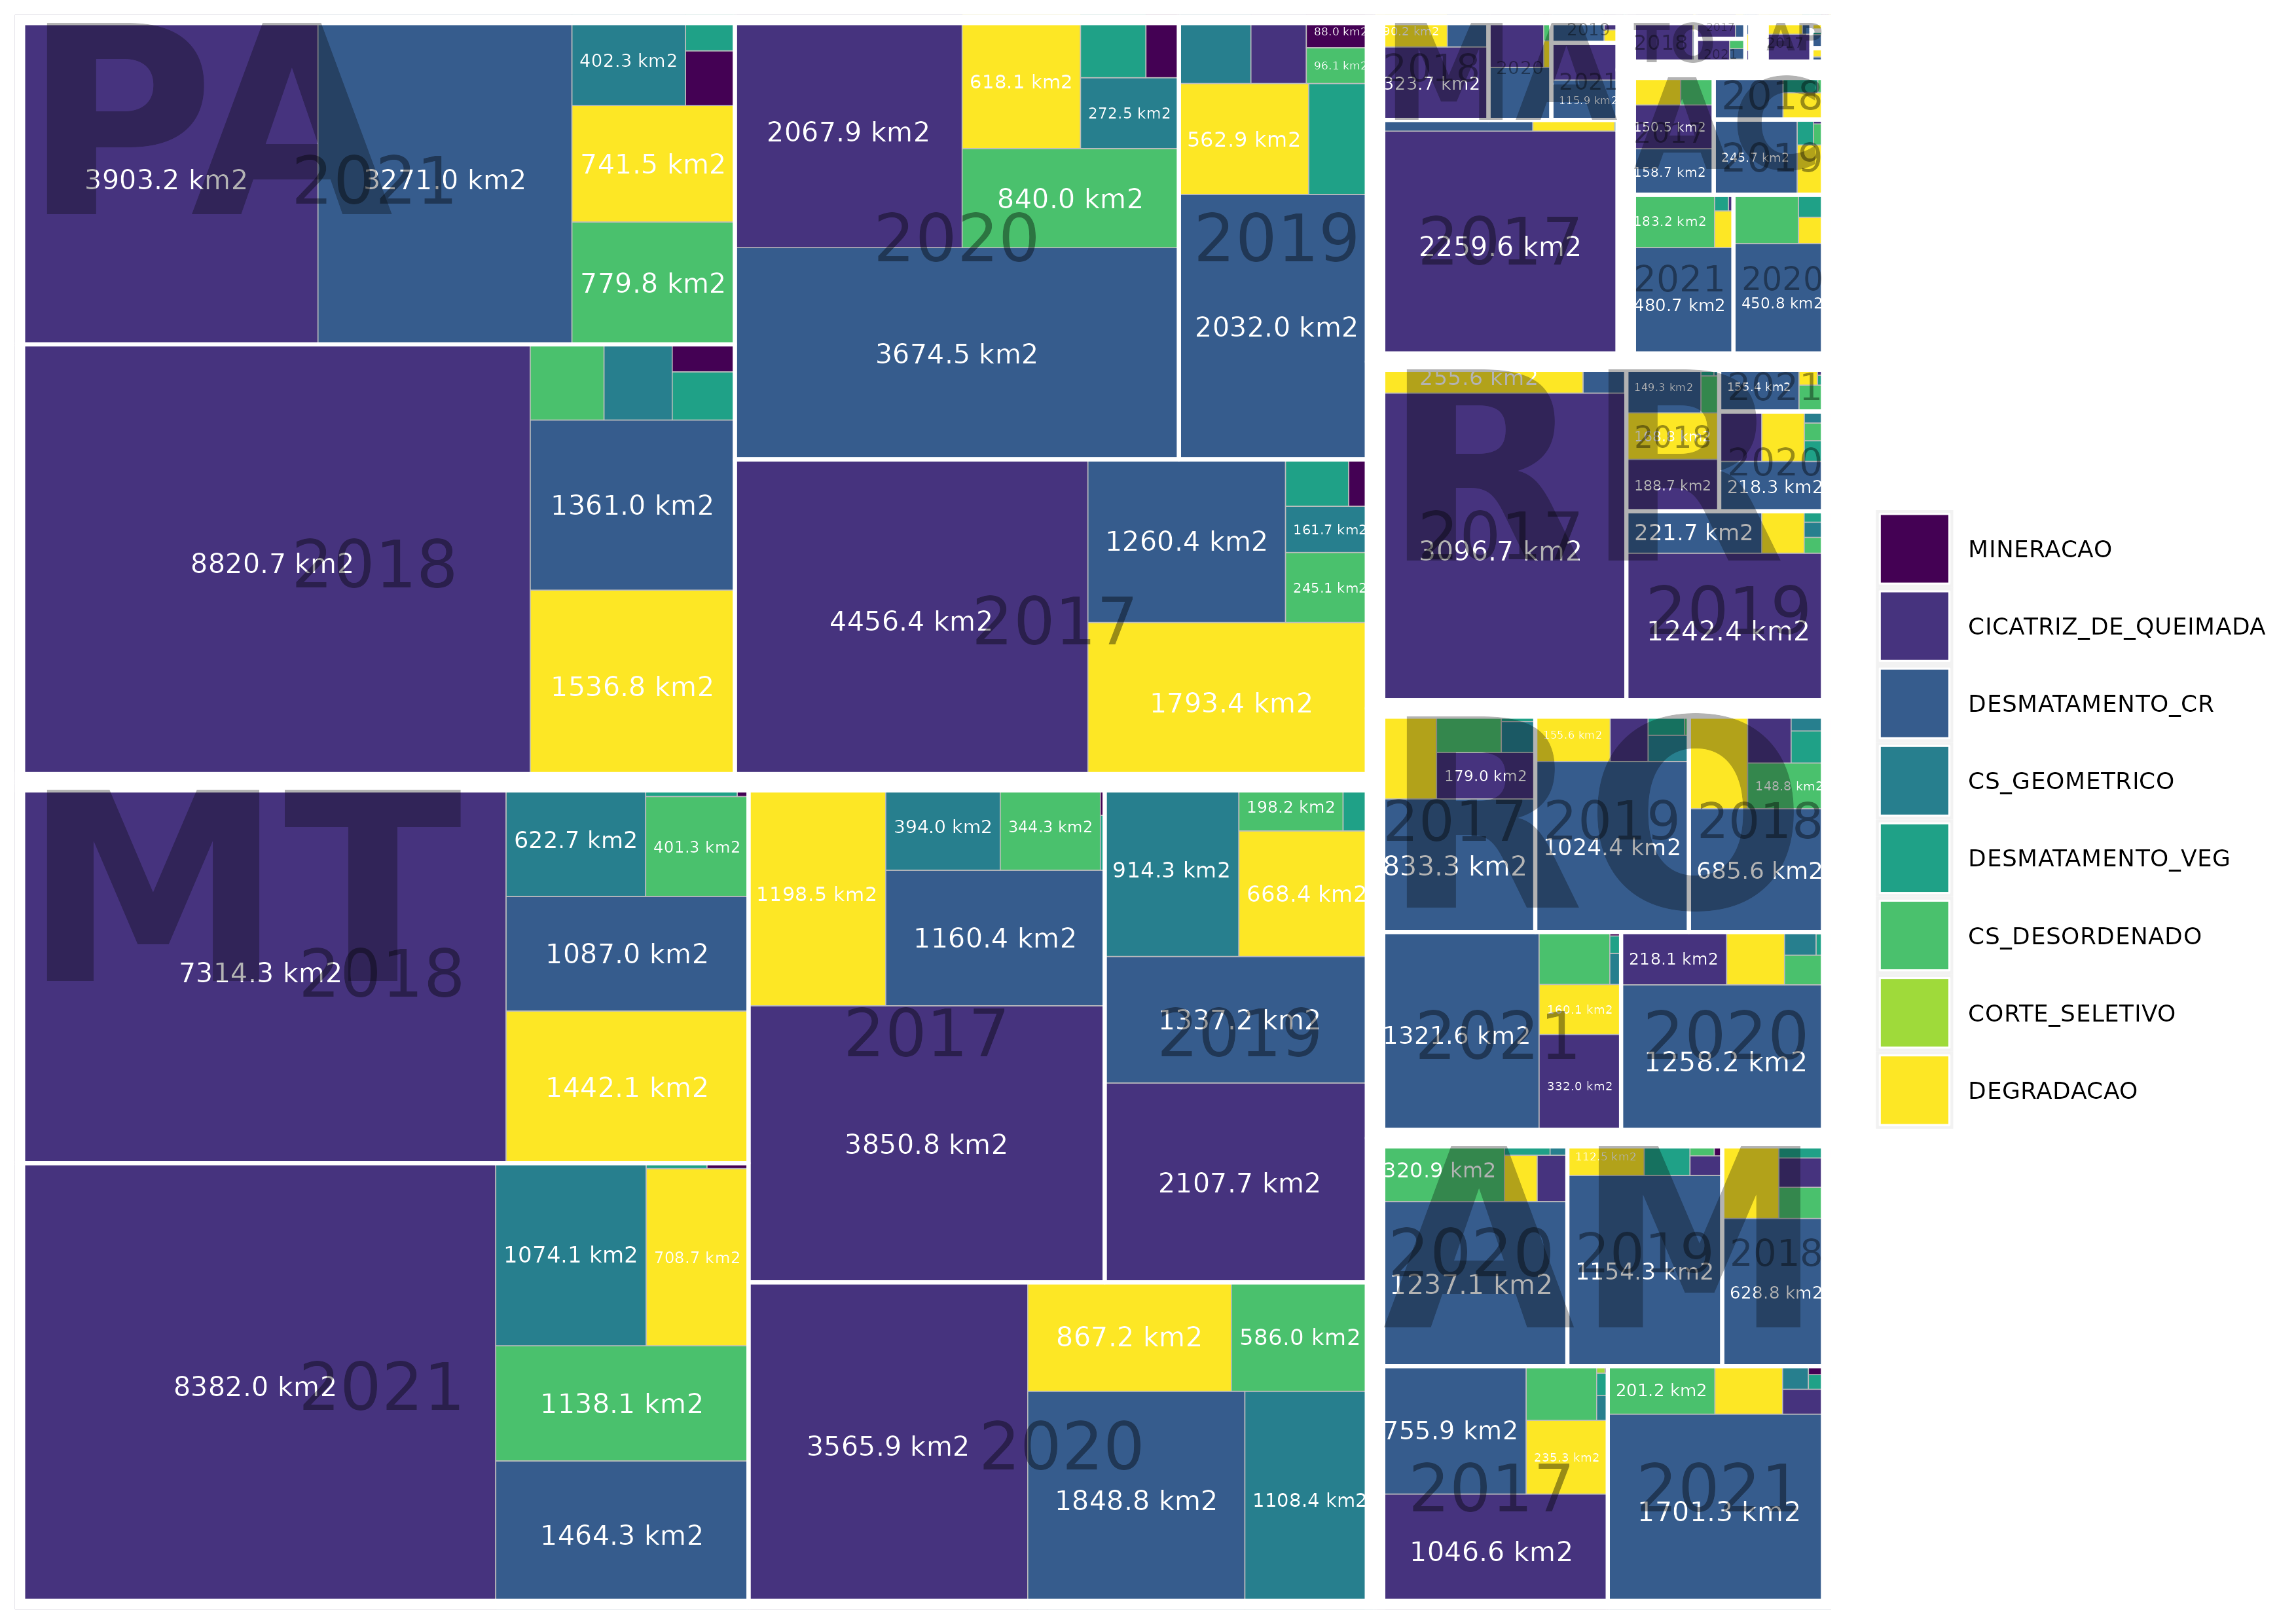
\includegraphics[width=0.75\linewidth]
        {./figures/plot_deter_area_by_state_pyear_type.png}
        \label{fig:deter_area_state_pyear_type}
    \end{figure}
\end{frame}

\begin{frame}
    \frametitle{DETER warnings and time}
    \begin{itemize}
        \item The spatial properties of DETER warning are inconsistent along 
            time (shape, size, position, orientation).
    \end{itemize}
\end{frame}

\begin{frame}
    \frametitle{Warnings are inconsistent along time}
    \begin{figure}[h] 
        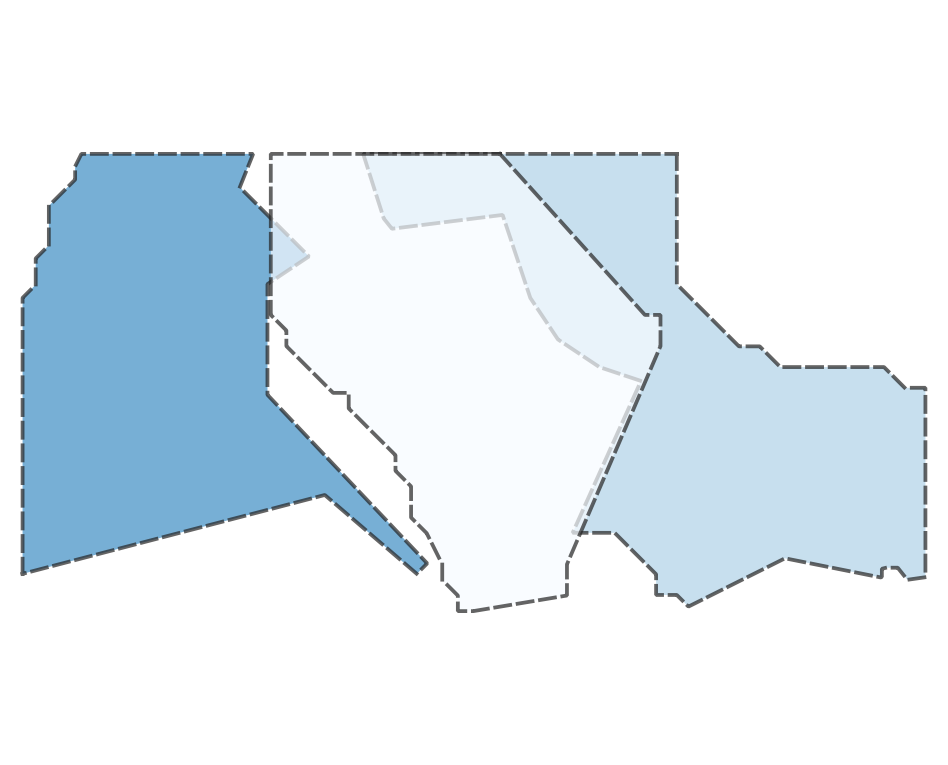
\includegraphics[width=0.60\linewidth]
        {./images/sample_deter_warnings.png}
        \label{fig:deter_subareas}
        \caption{DETER warnings don't fit along time.}
    \end{figure}
\end{frame}


%---- DETER subareas ----

\begin{frame}
    \frametitle{DETER subareas}
    \begin{itemize}
        \item The spatial properties of DETER warning are inconsistent along 
            time (shape, size, area, position).
        \item DETER subareas maintain their spatial properties along time.
    \end{itemize}
\end{frame}

\begin{frame}
    \frametitle{DETER subareas}
    \begin{figure}[h] 
        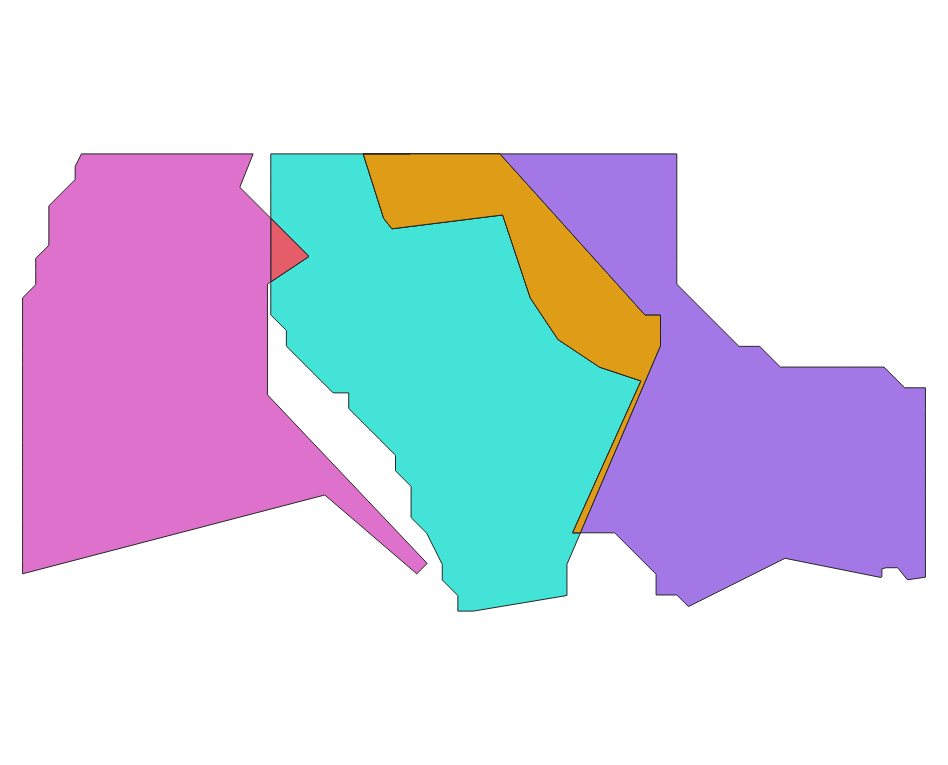
\includegraphics[width=0.60\linewidth]
        {./images/sample_deter_subareas.png}
        \caption{From 3 DETER we get 7 subareas!}
        \label{fig:deter_subareas}
    \end{figure}
\end{frame}

\begin{frame}
    \frametitle{DETER subareas}
    \begin{figure}[h] 
        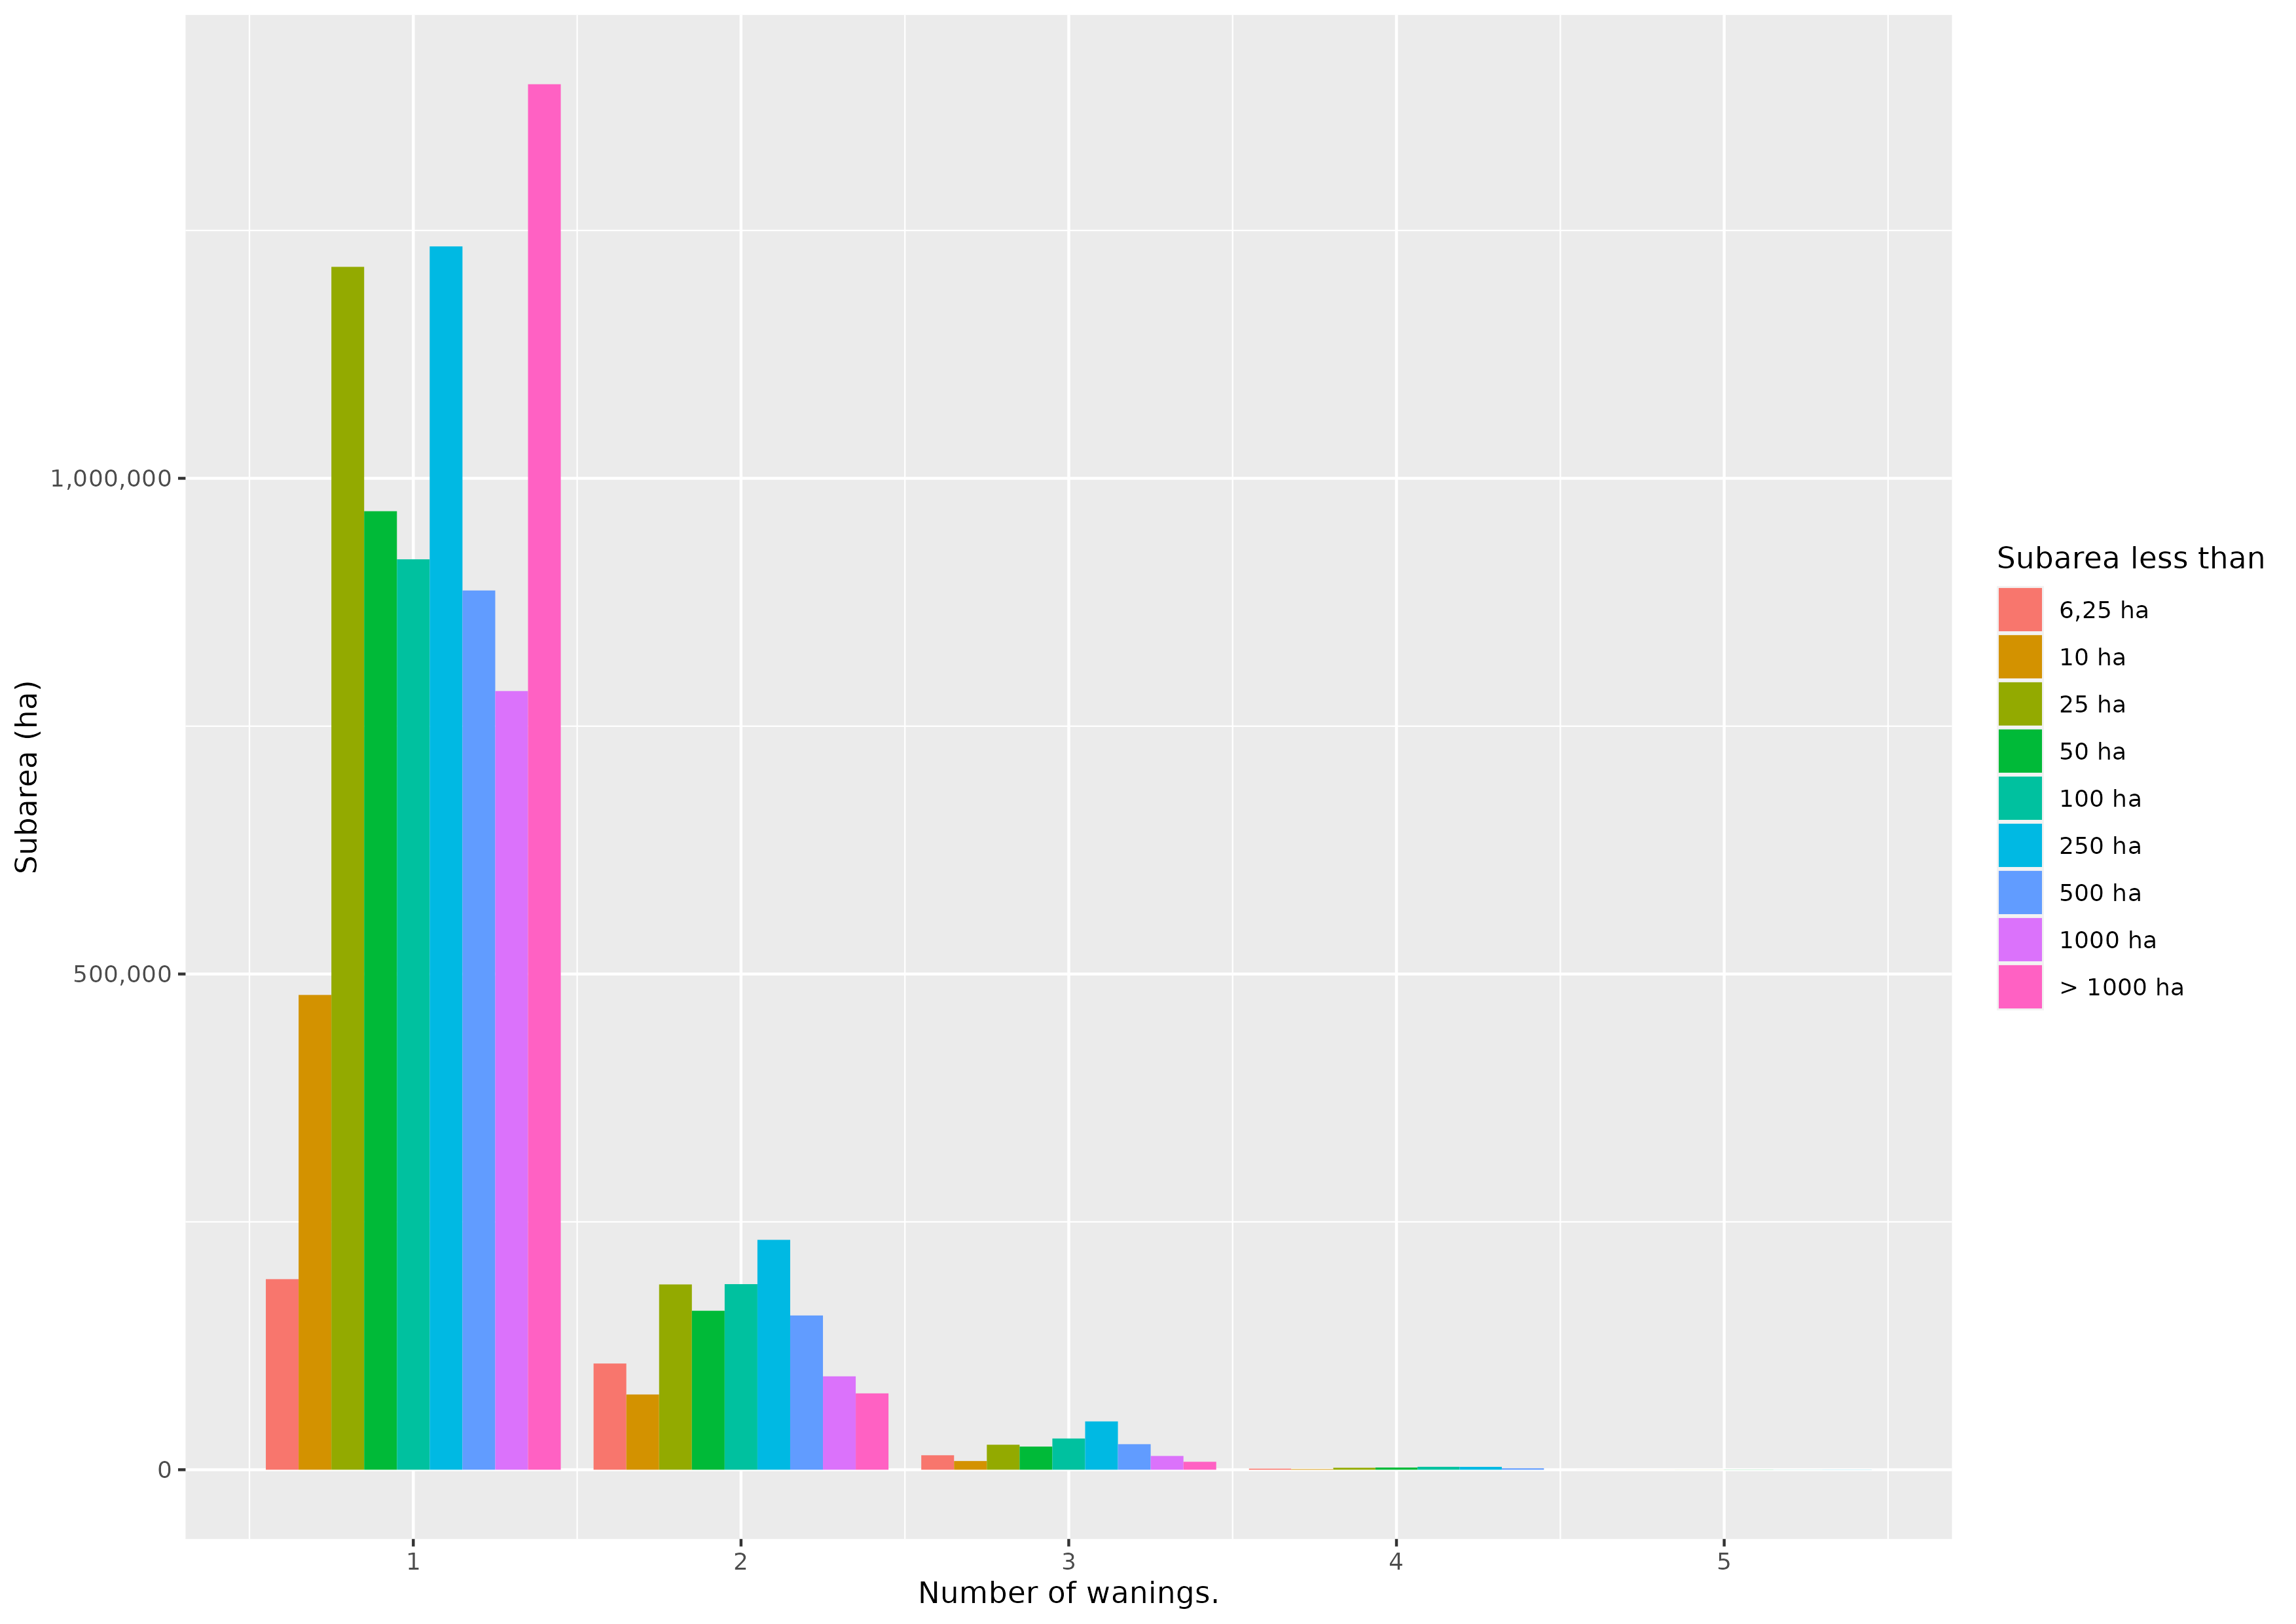
\includegraphics[width=0.65\linewidth]
        {./figures/plot_deter_subarea_by_nwarnings.png}
        \caption{There are subareas with up to 5 recurrent warnings.}
        \label{fig:deter_subareas_nwarnings}
    \end{figure}
\end{frame}

\begin{frame}
    \frametitle{DETER subareas}
    \begin{figure}[h] 
        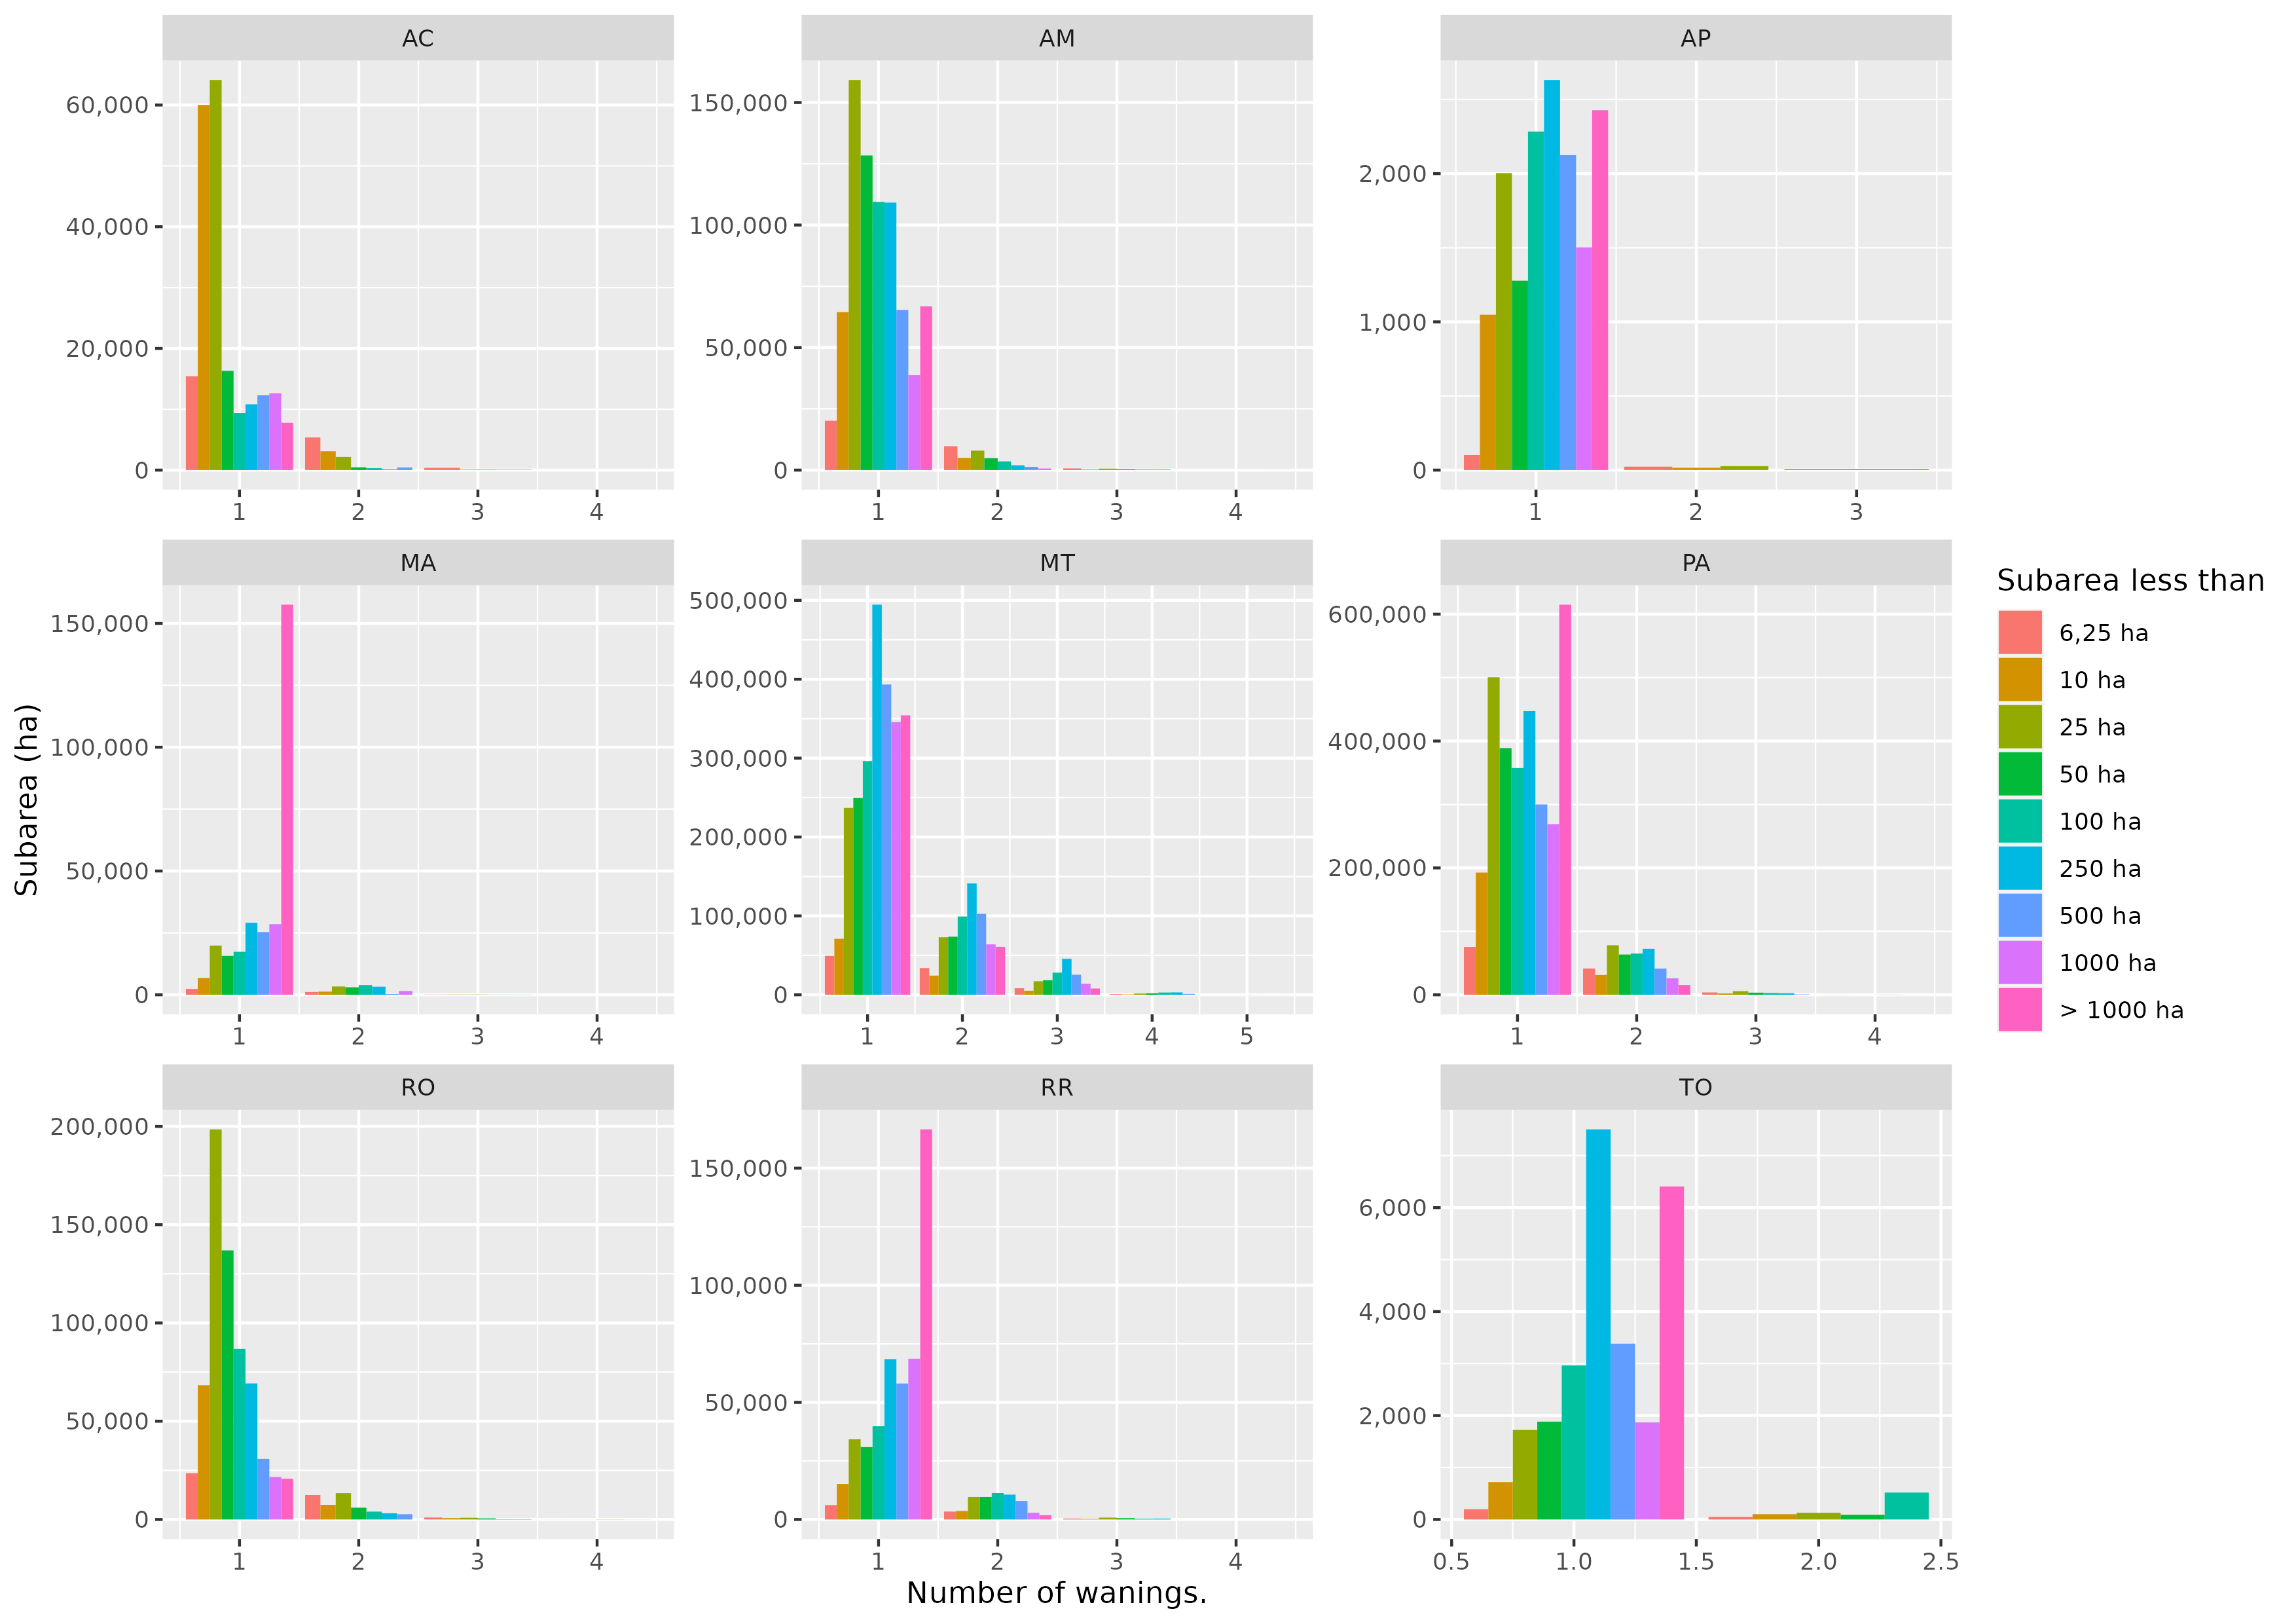
\includegraphics[width=0.65\linewidth]
        {./figures/plot_deter_subarea_by_warnings_state.png}
        \caption{The warning recurrence changes by brazilian state.}
        \label{fig:deter_subarea_warnings_state}
    \end{figure}
\end{frame}

\begin{frame}
    \frametitle{DETER subareas}
    \begin{figure}[h] 
        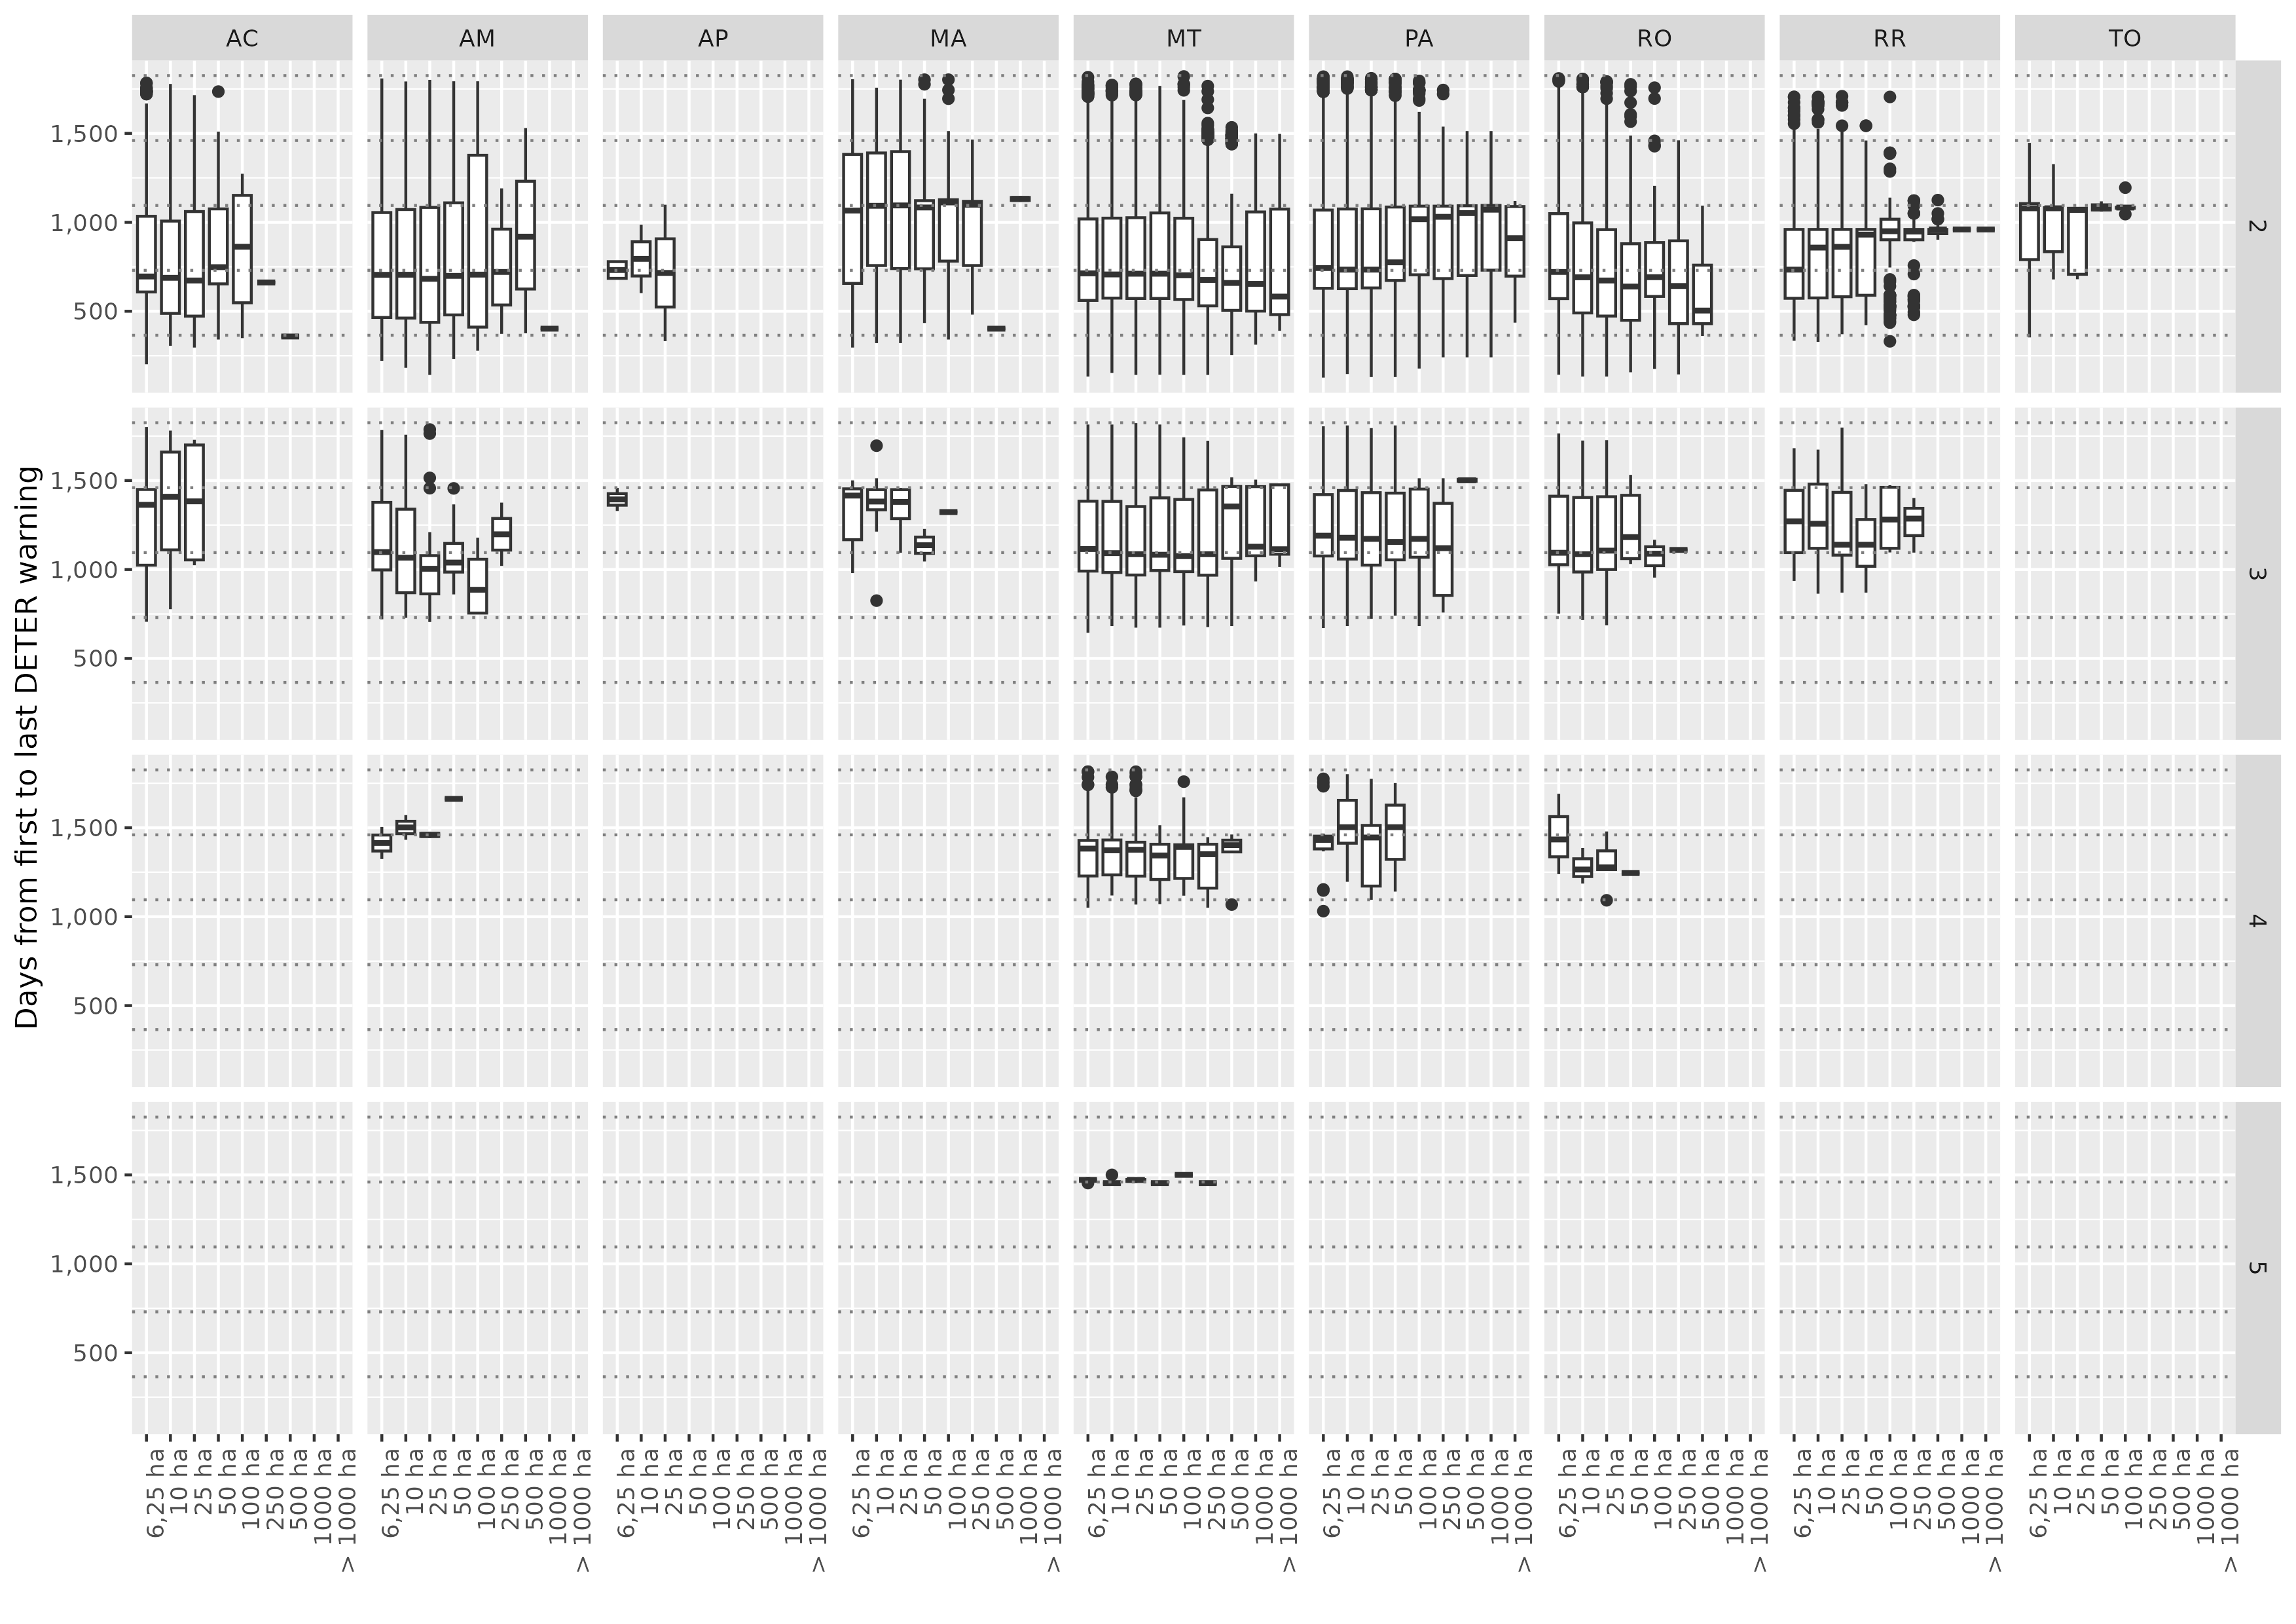
\includegraphics[width=0.65\linewidth]
        {./figures/plot_deter_days_first_to_last.png}
        \caption{Number of days between first and last warning.}
        \label{fig:deter_days_first_to_last}
    \end{figure}
\end{frame}

\begin{frame}
    \frametitle{DETER subareas}
    \begin{figure}[h] 
        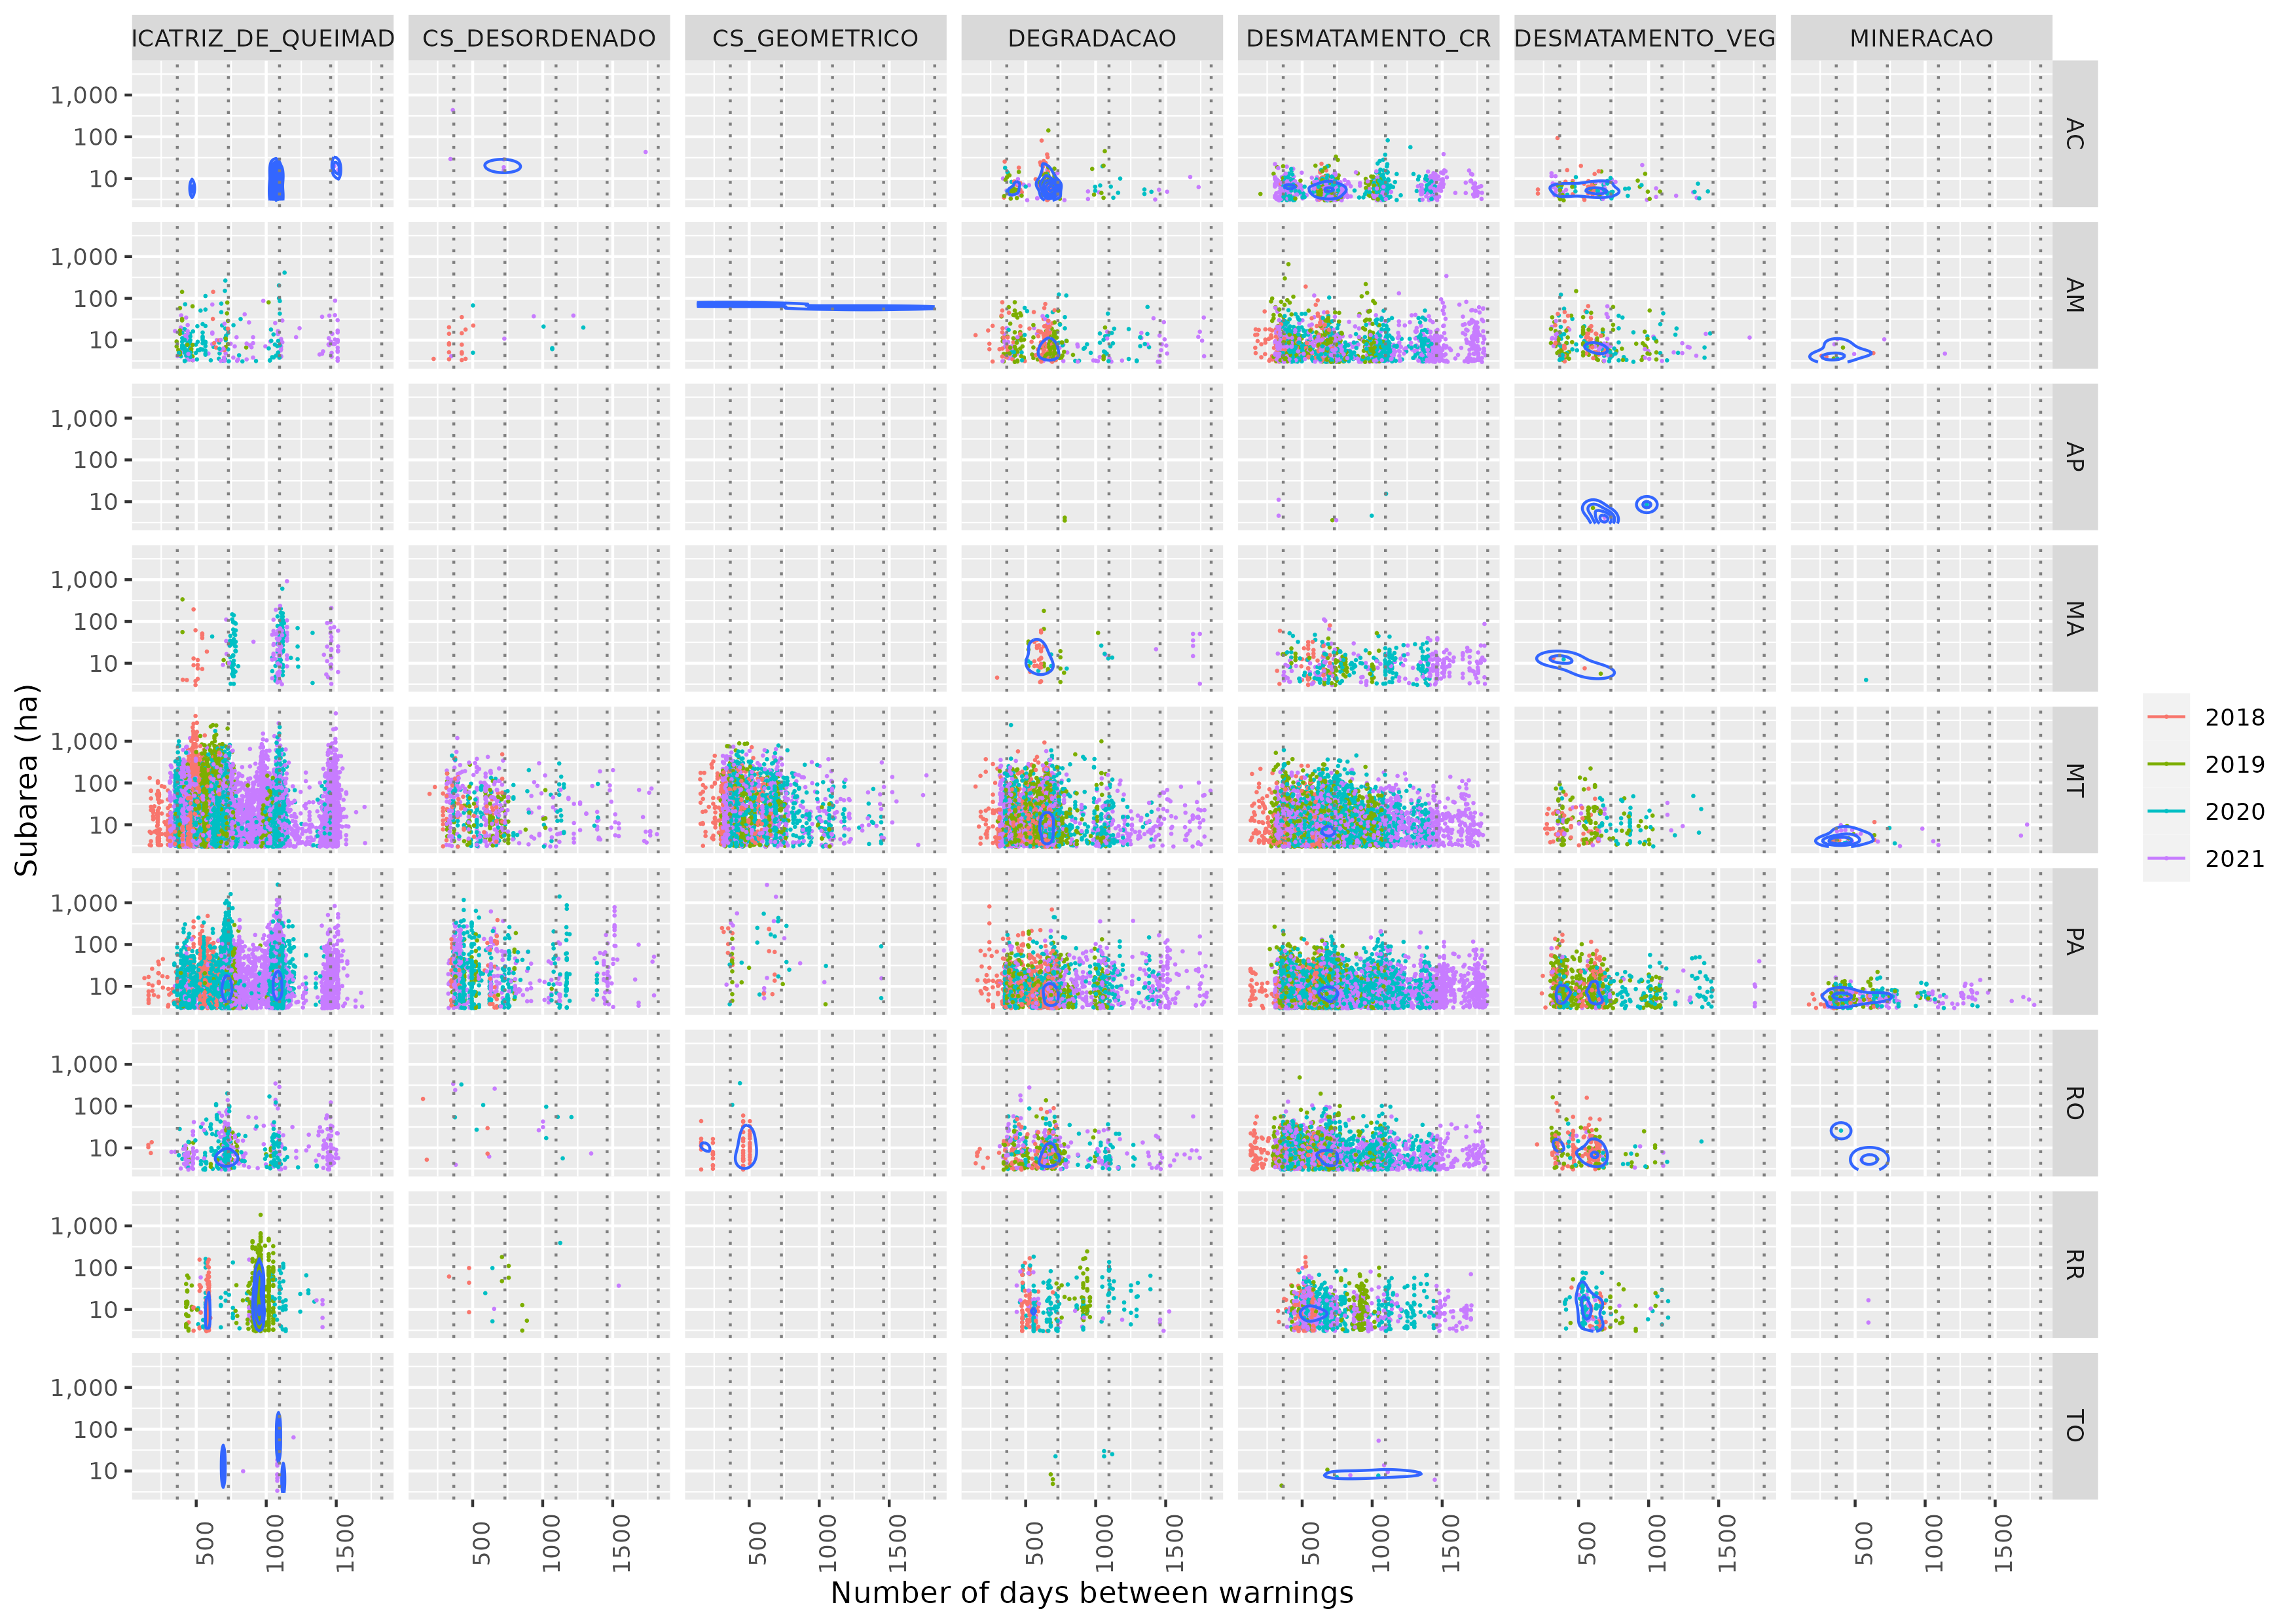
\includegraphics[width=0.65\linewidth]
        {./figures/plot_deter_subarea_density_by_state_first-type_nwarnings.png}
        \caption{The number of days between warnings behavious in space and 
        time.}
        \label{fig:deter_subarea_density_state_first_type_nwarnings}
    \end{figure}
\end{frame}

\begin{frame}
    \frametitle{DETER subareas}
    \begin{figure}[h] 
        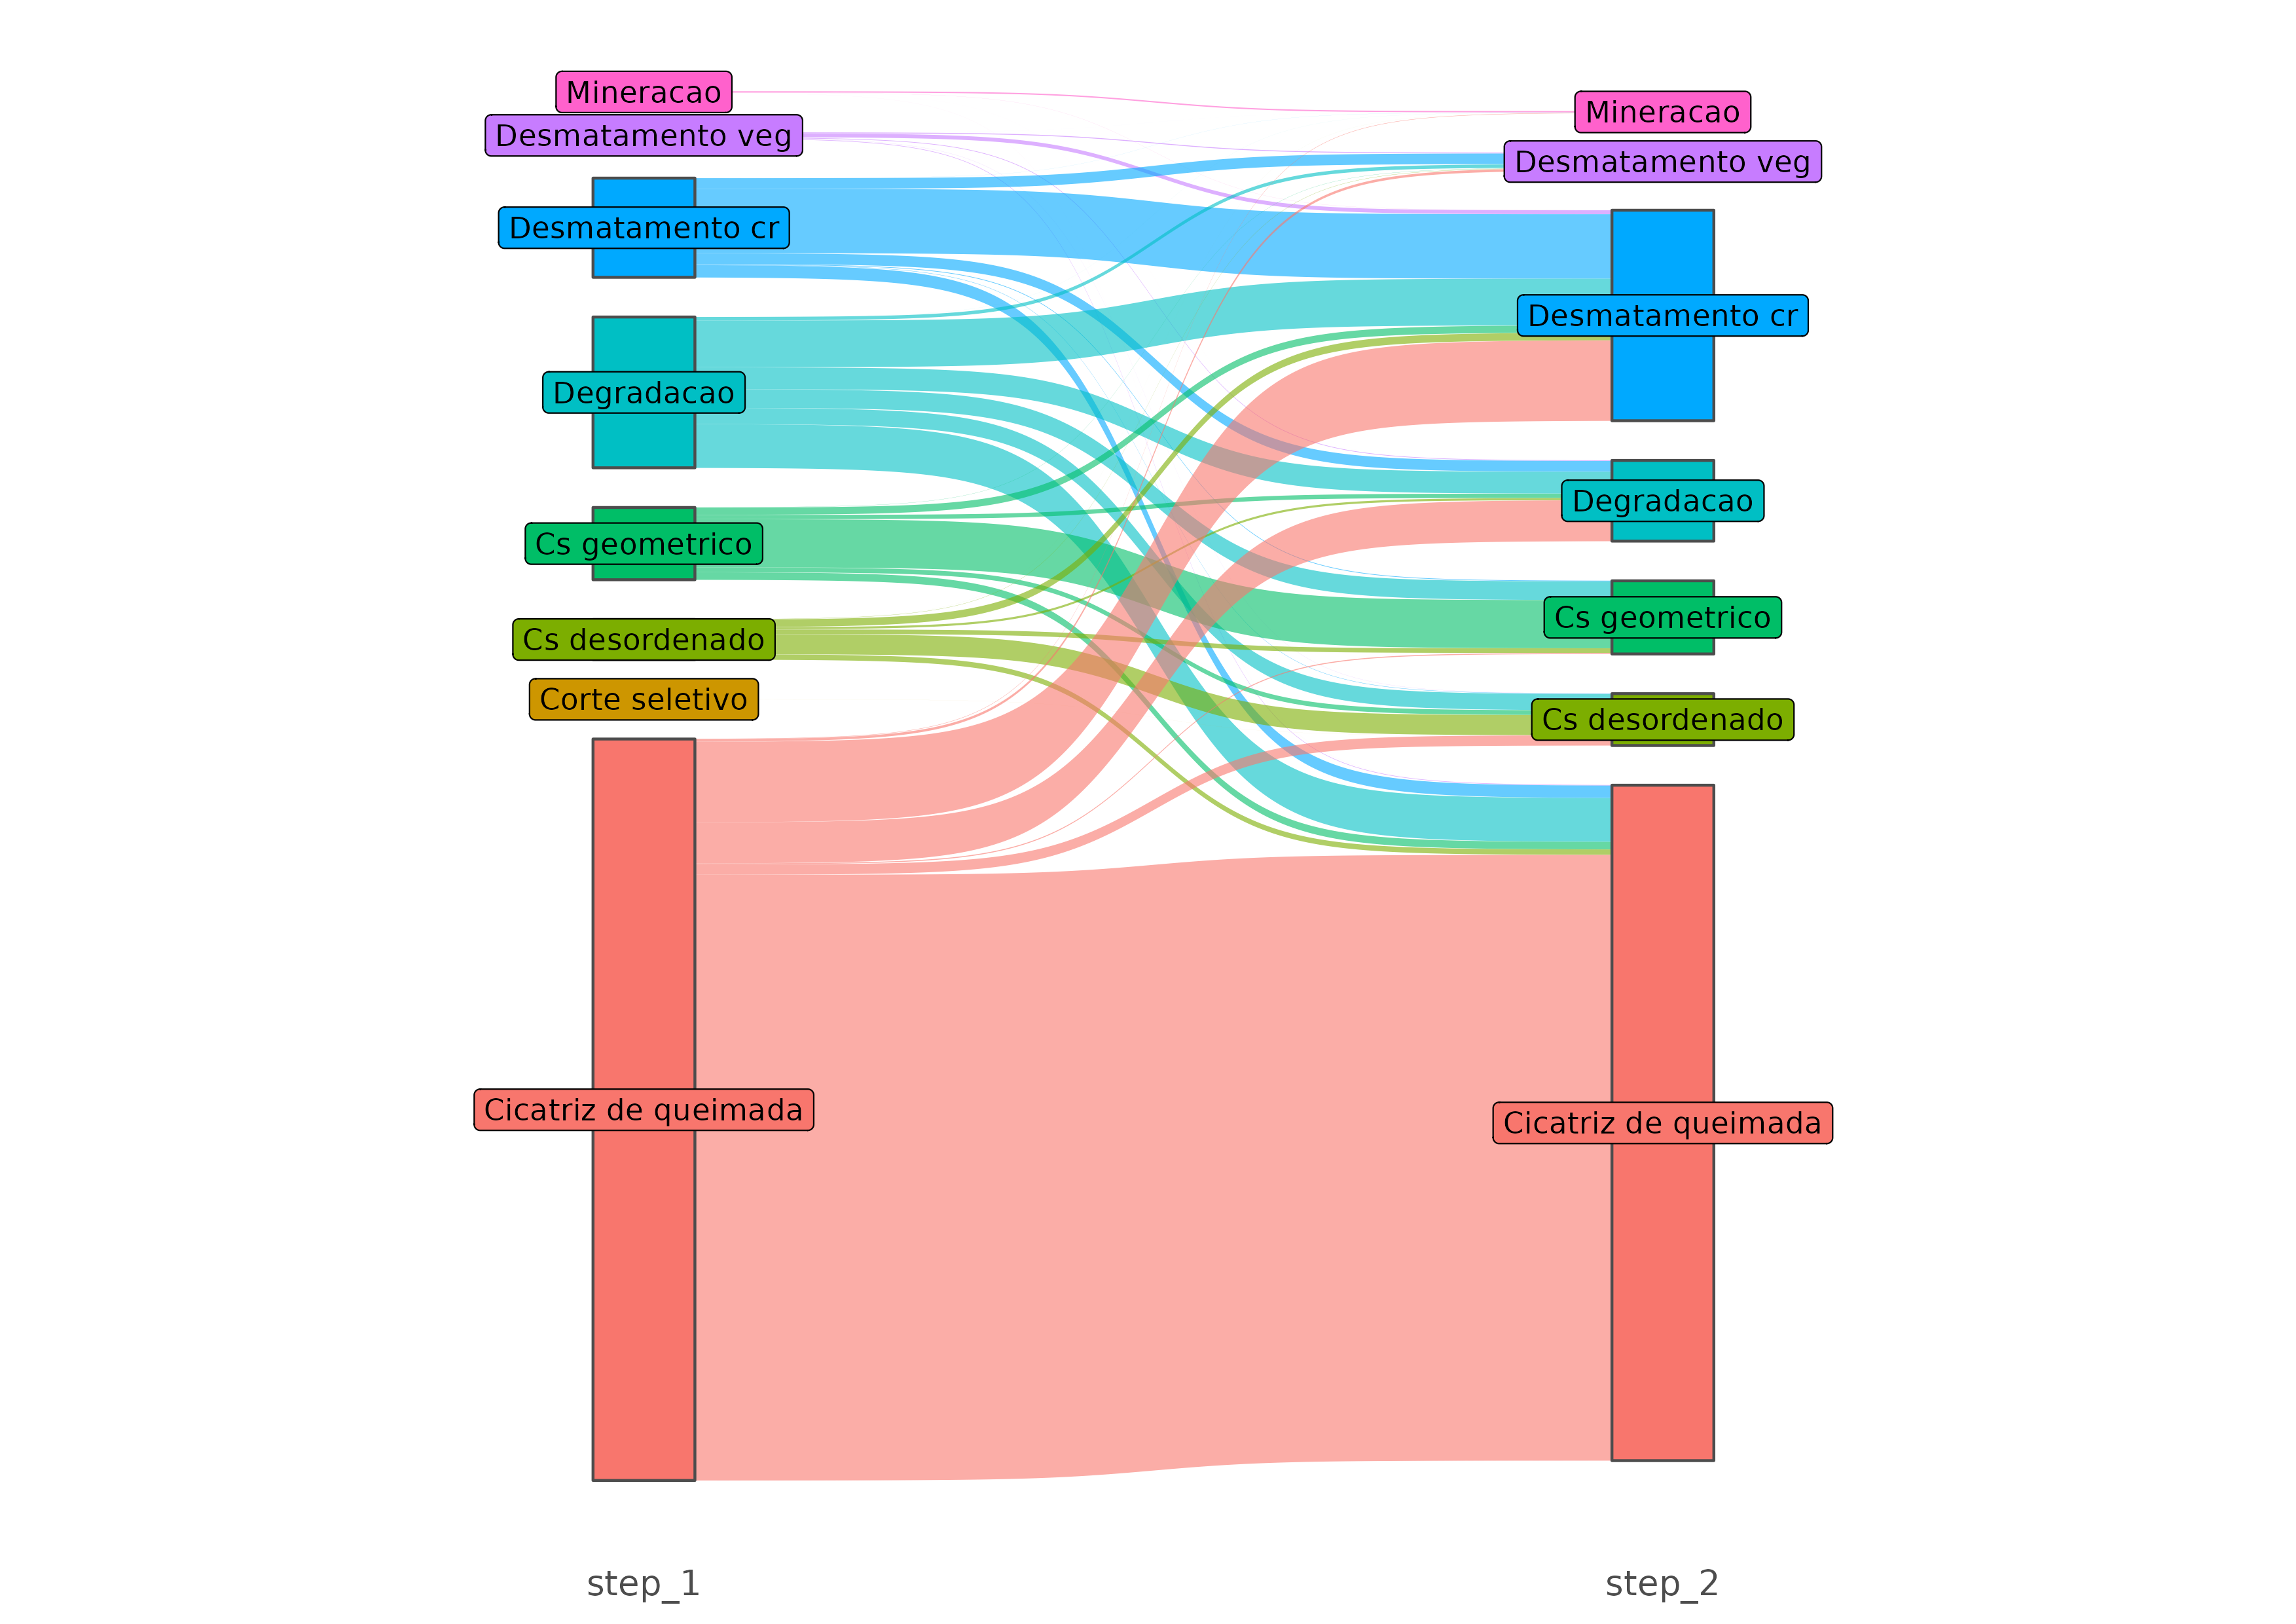
\includegraphics[width=0.65\linewidth]
        {./figures/plot_deter_subarea_trajectory_2.png}
        \caption{Tajectory of subareas with 2 wanings.}
        \label{fig:deter_subarea_trajectory_2}
    \end{figure}
\end{frame}

\begin{frame}
    \frametitle{DETER subareas}
    \begin{figure}[h] 
        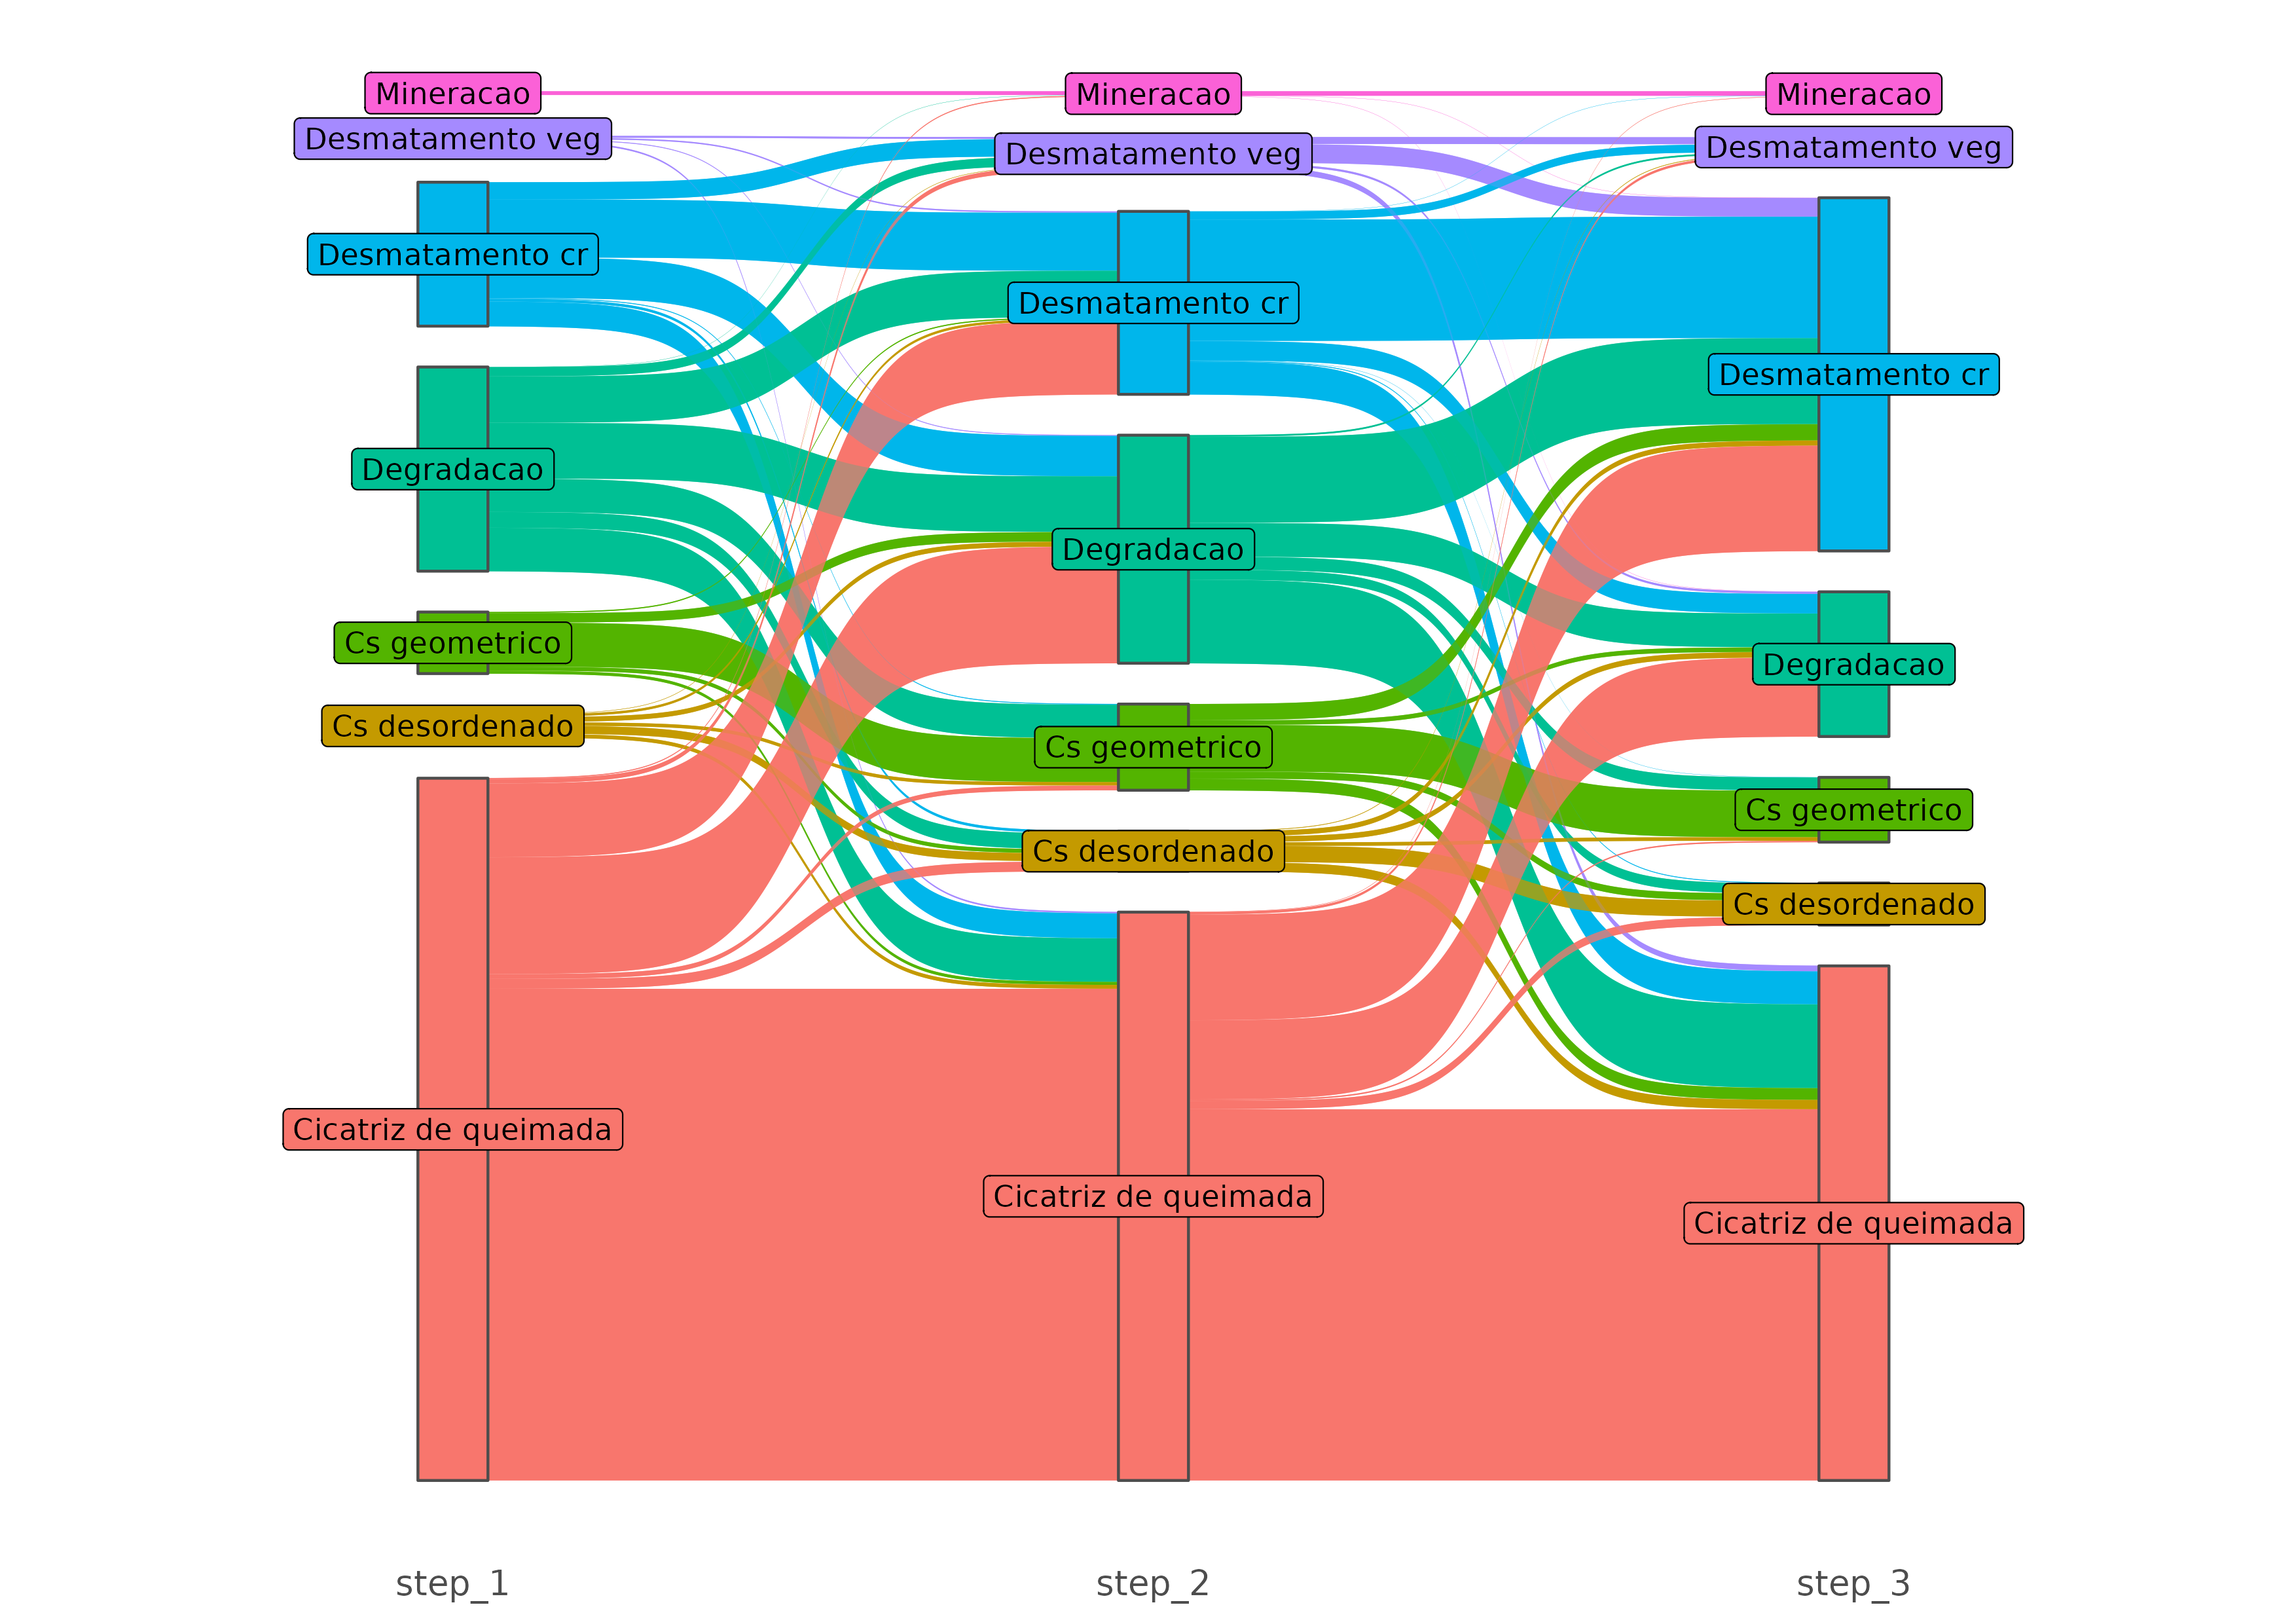
\includegraphics[width=0.65\linewidth]
        {./figures/plot_deter_subarea_trajectory_3.png}
        \caption{Tajectory of subareas with 3 wanings.}
        \label{fig:deter_subarea_trajectory_3}
    \end{figure}
\end{frame}

\begin{frame}
    \frametitle{DETER subareas}
    \begin{figure}[h] 
        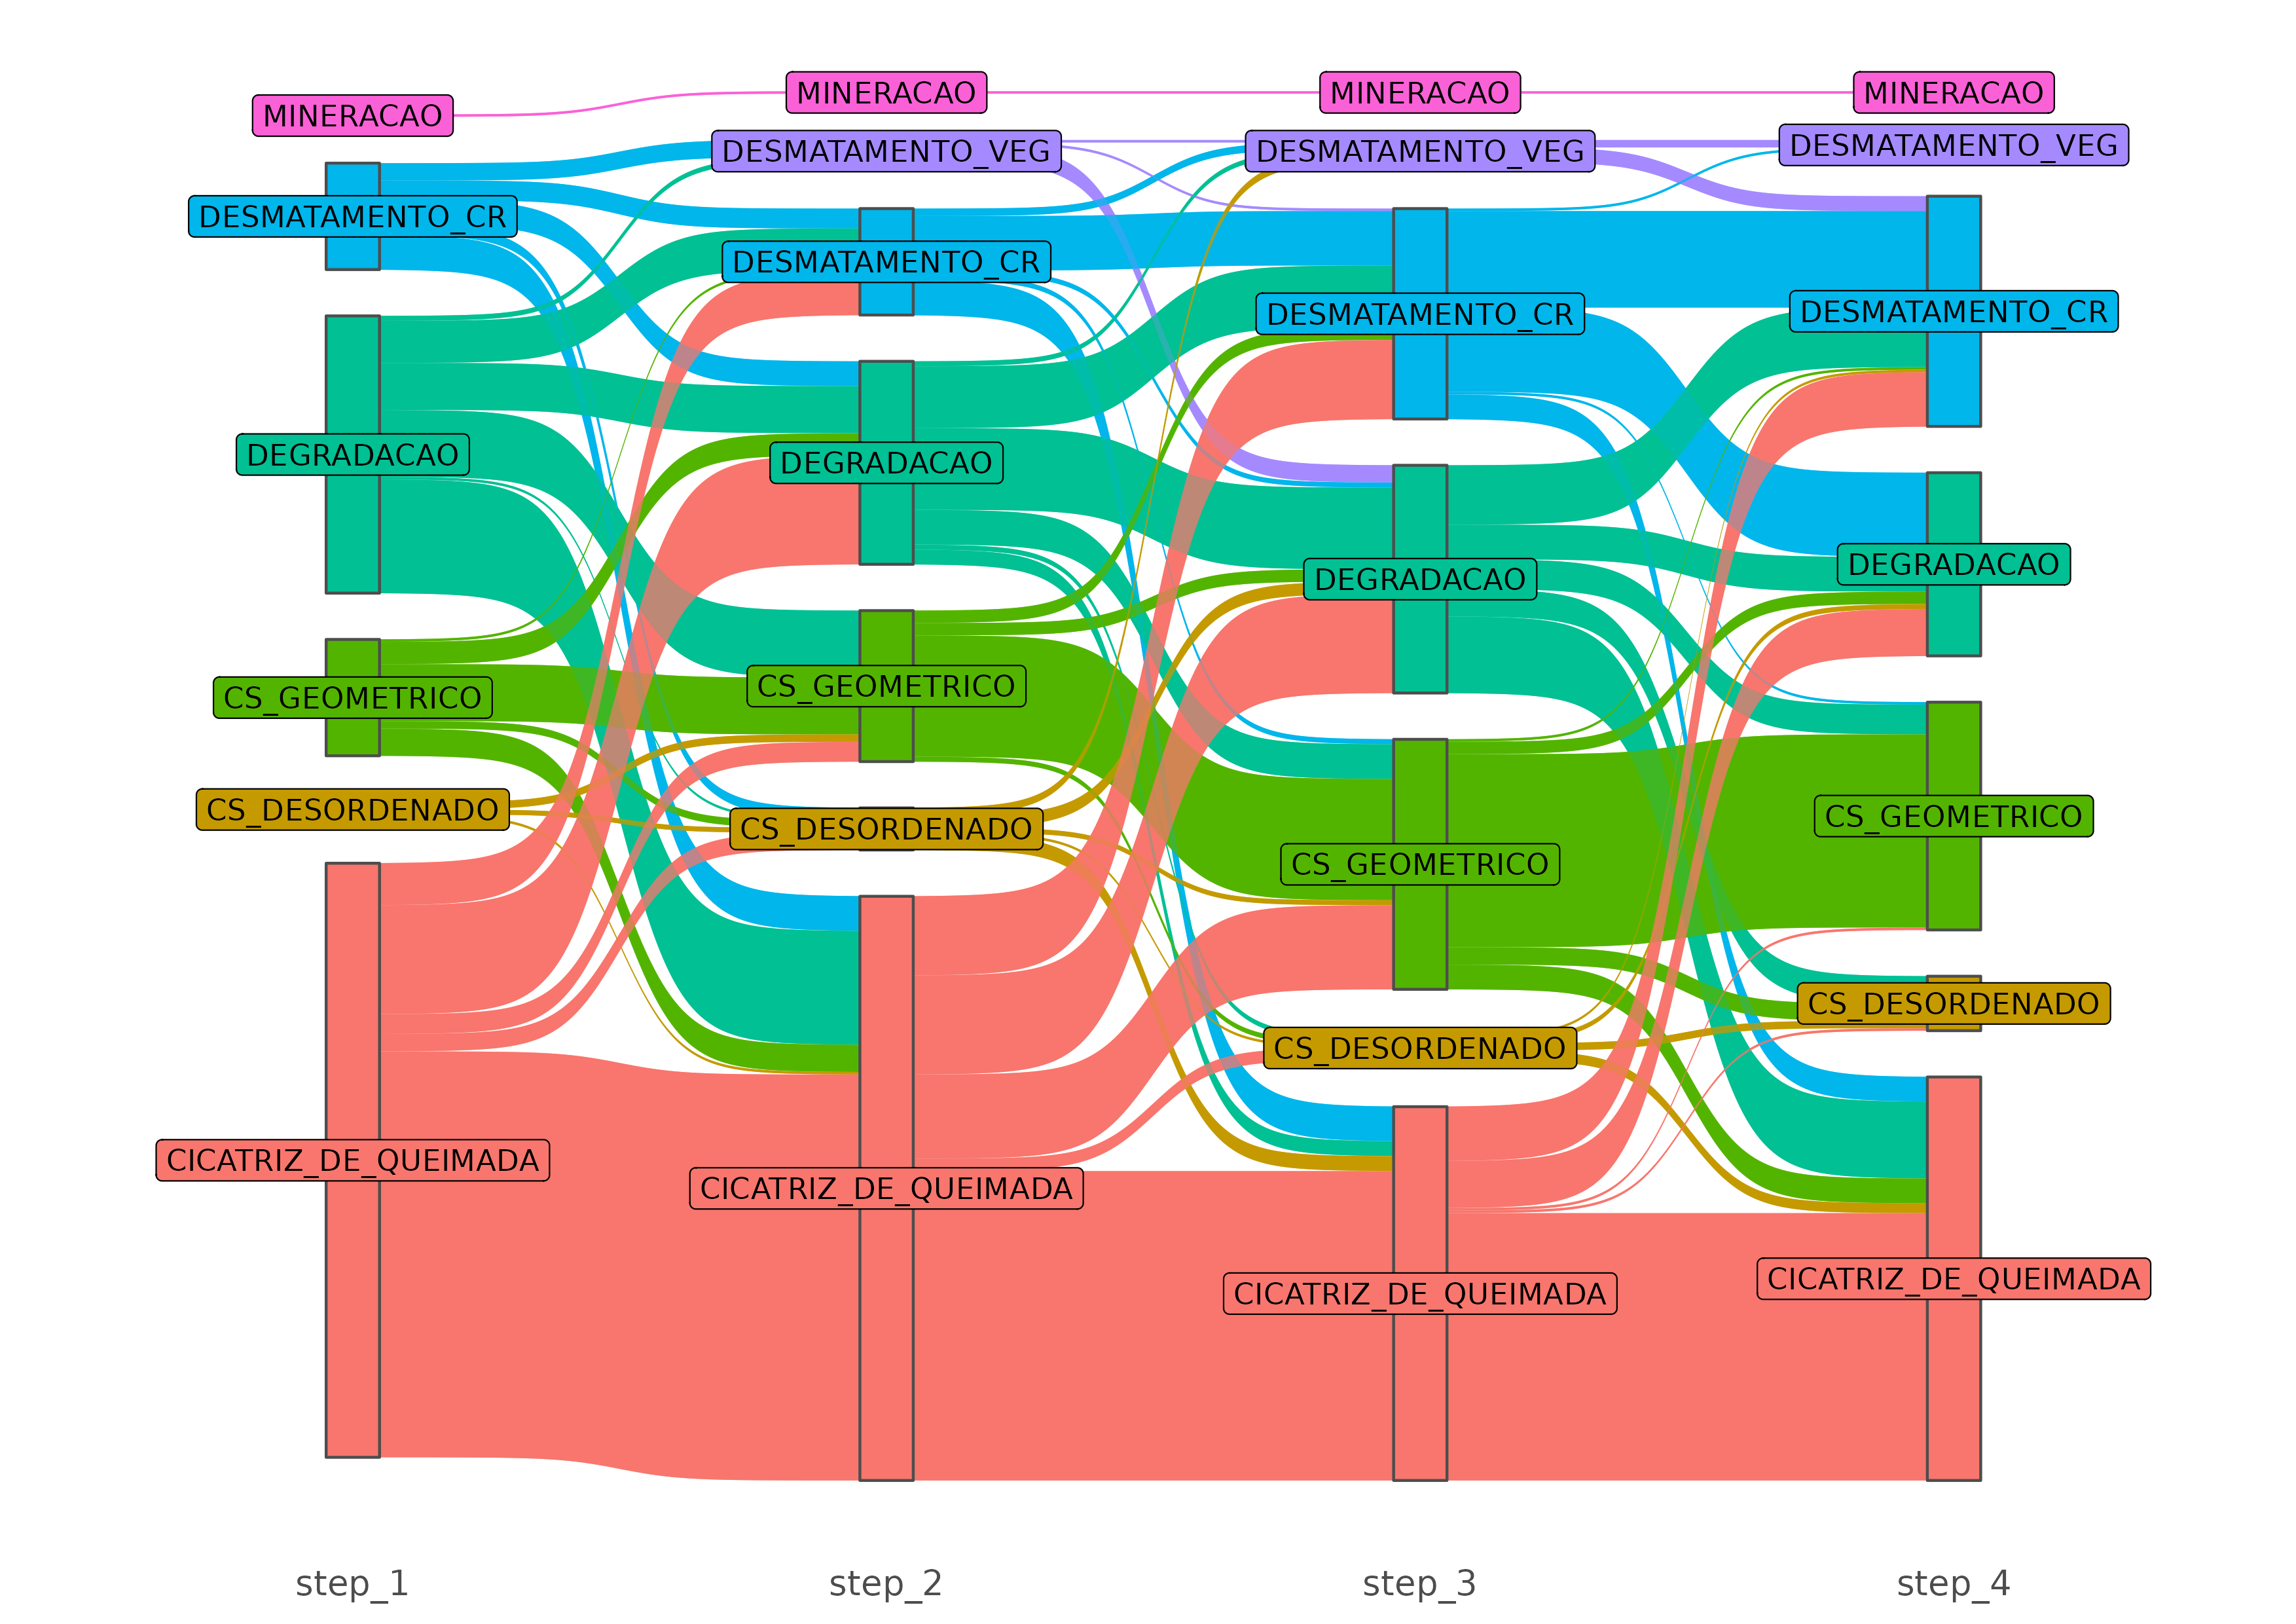
\includegraphics[width=0.65\linewidth]
        {./figures/plot_deter_subarea_trajectory_4.png}
        \caption{Tajectory of subareas with 4 wanings.}
        \label{fig:deter_subarea_trajectory_4}
    \end{figure}
\end{frame}

\begin{frame}
    \frametitle{DETER subareas}
    \begin{figure}[h] 
        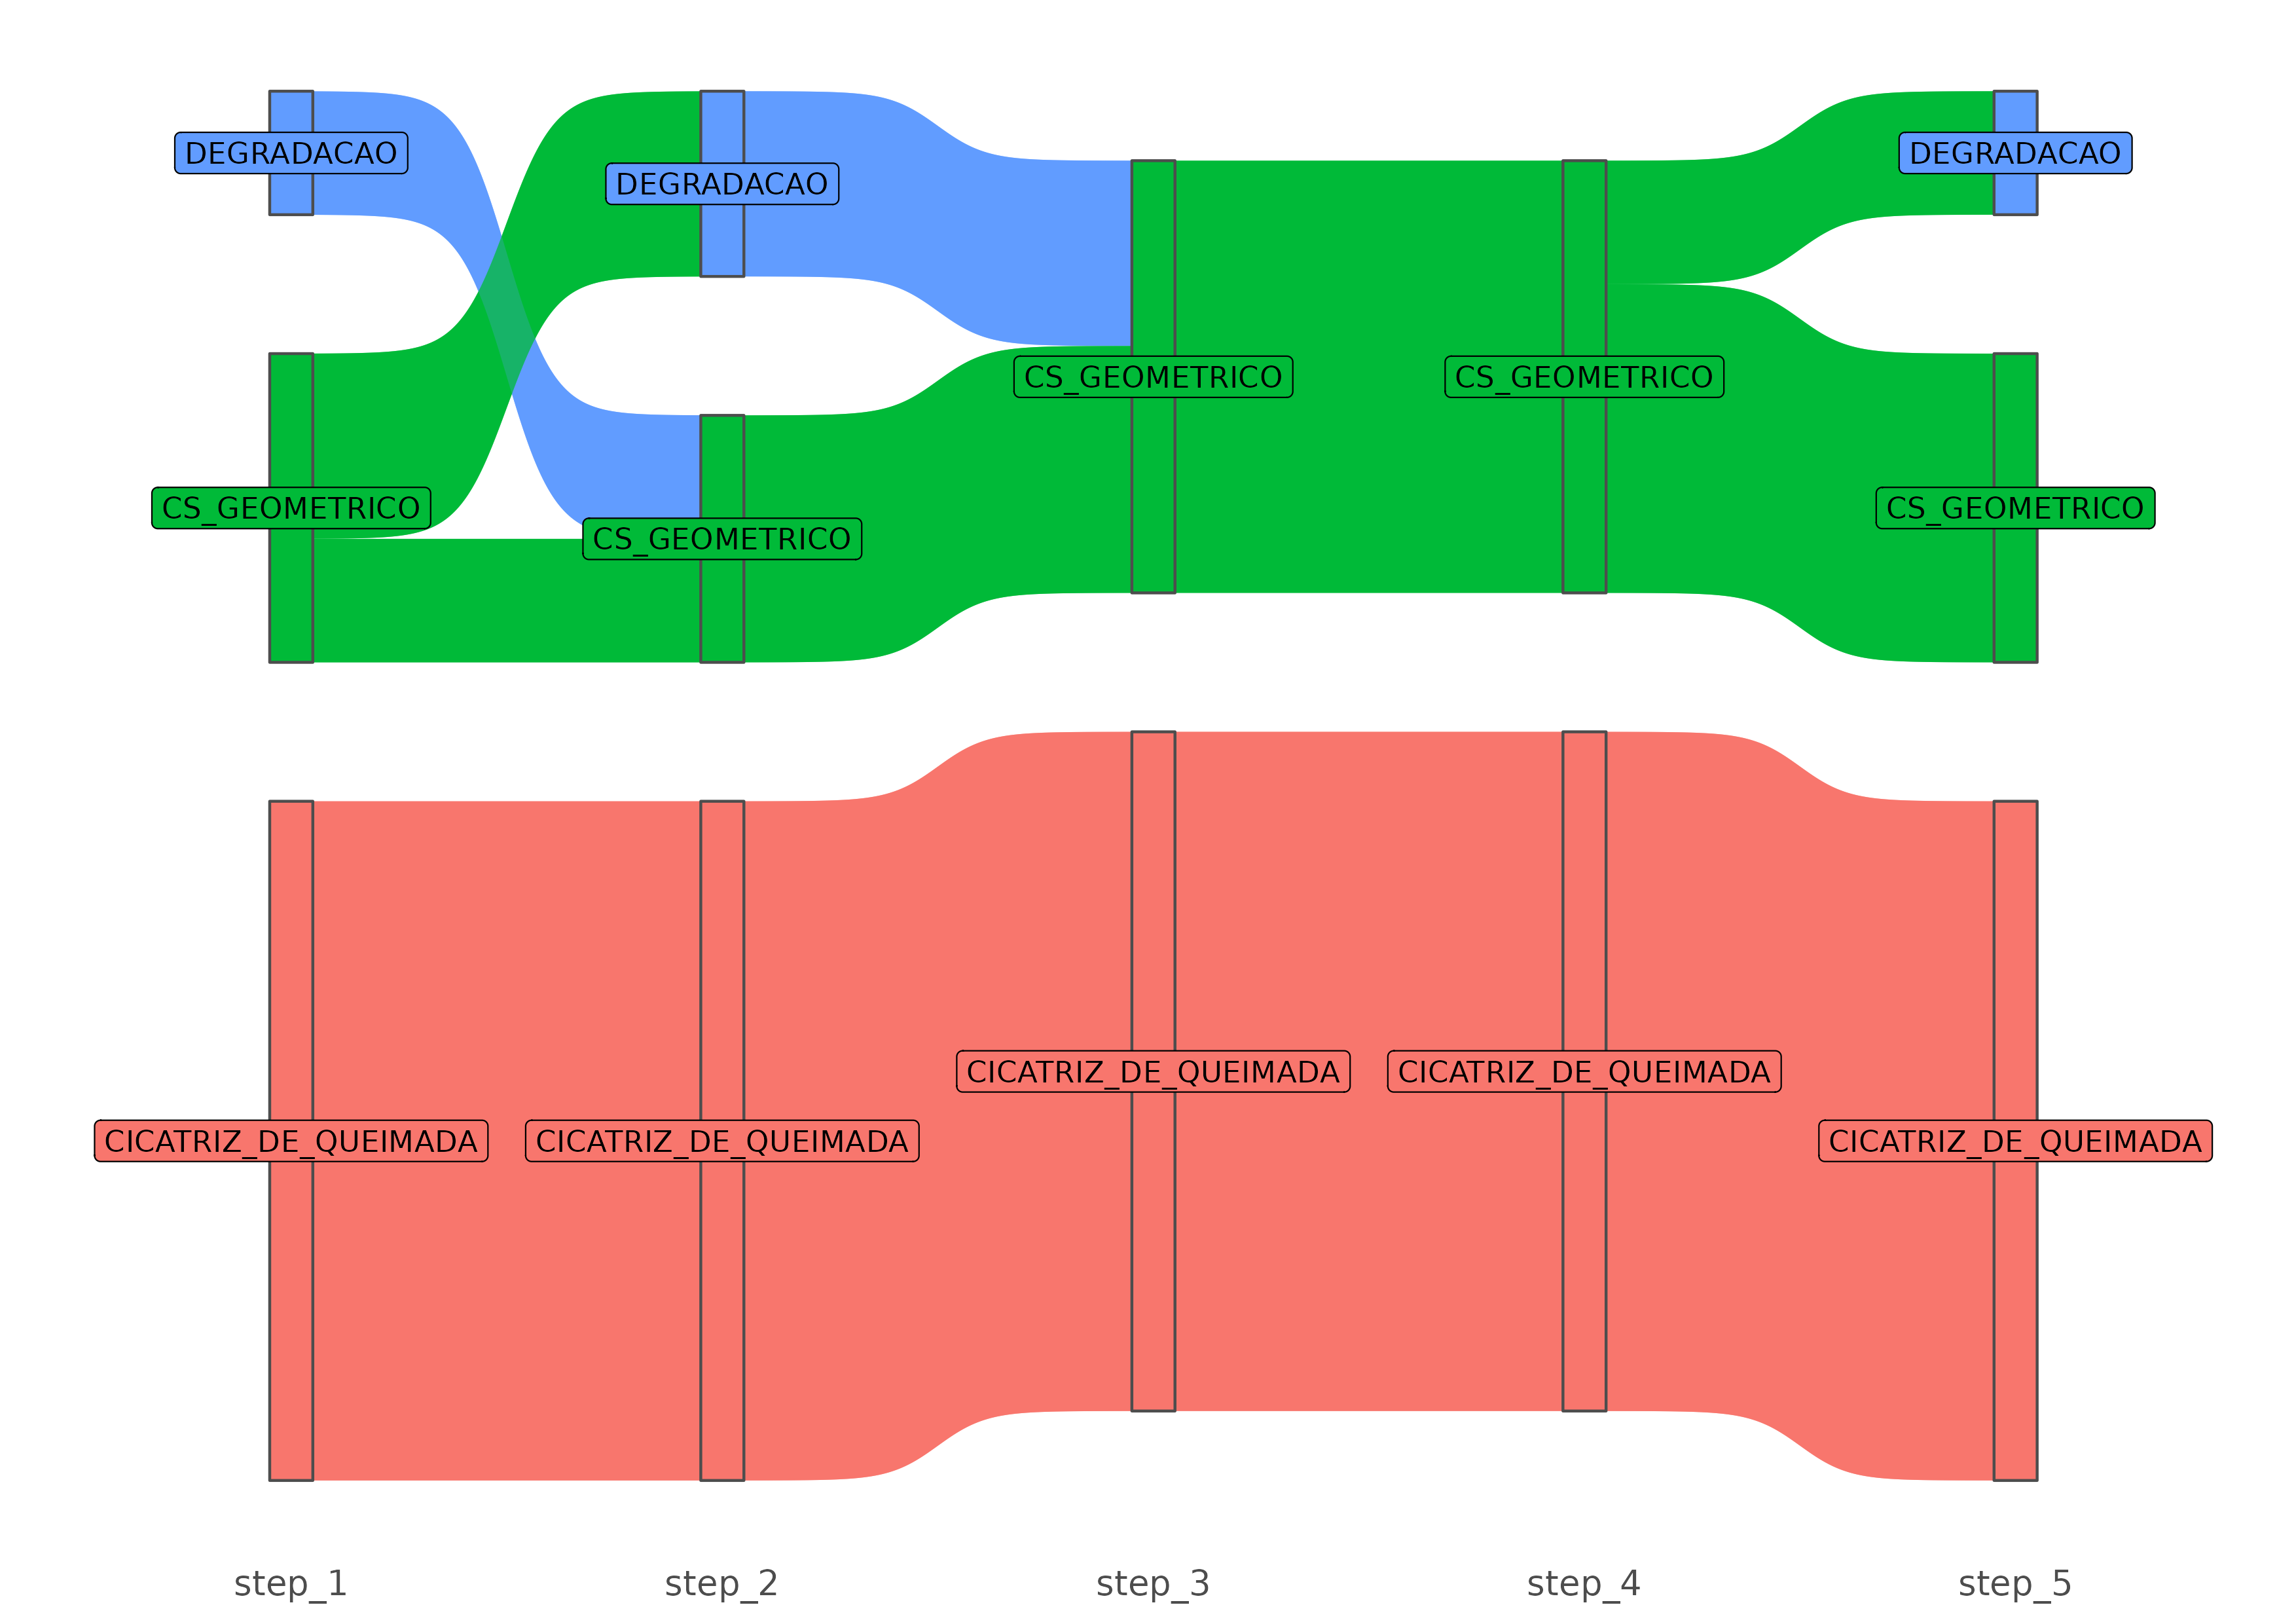
\includegraphics[width=0.65\linewidth]
        {./figures/plot_deter_subarea_trajectory_5.png}
        \caption{Tajectory of subareas with 5 wanings.}
        \label{fig:deter_subarea_trajectory_5}
    \end{figure}
\end{frame}

\begin{frame}
    \frametitle{DETER - PRODES subareas}
    \begin{figure}[h] 
        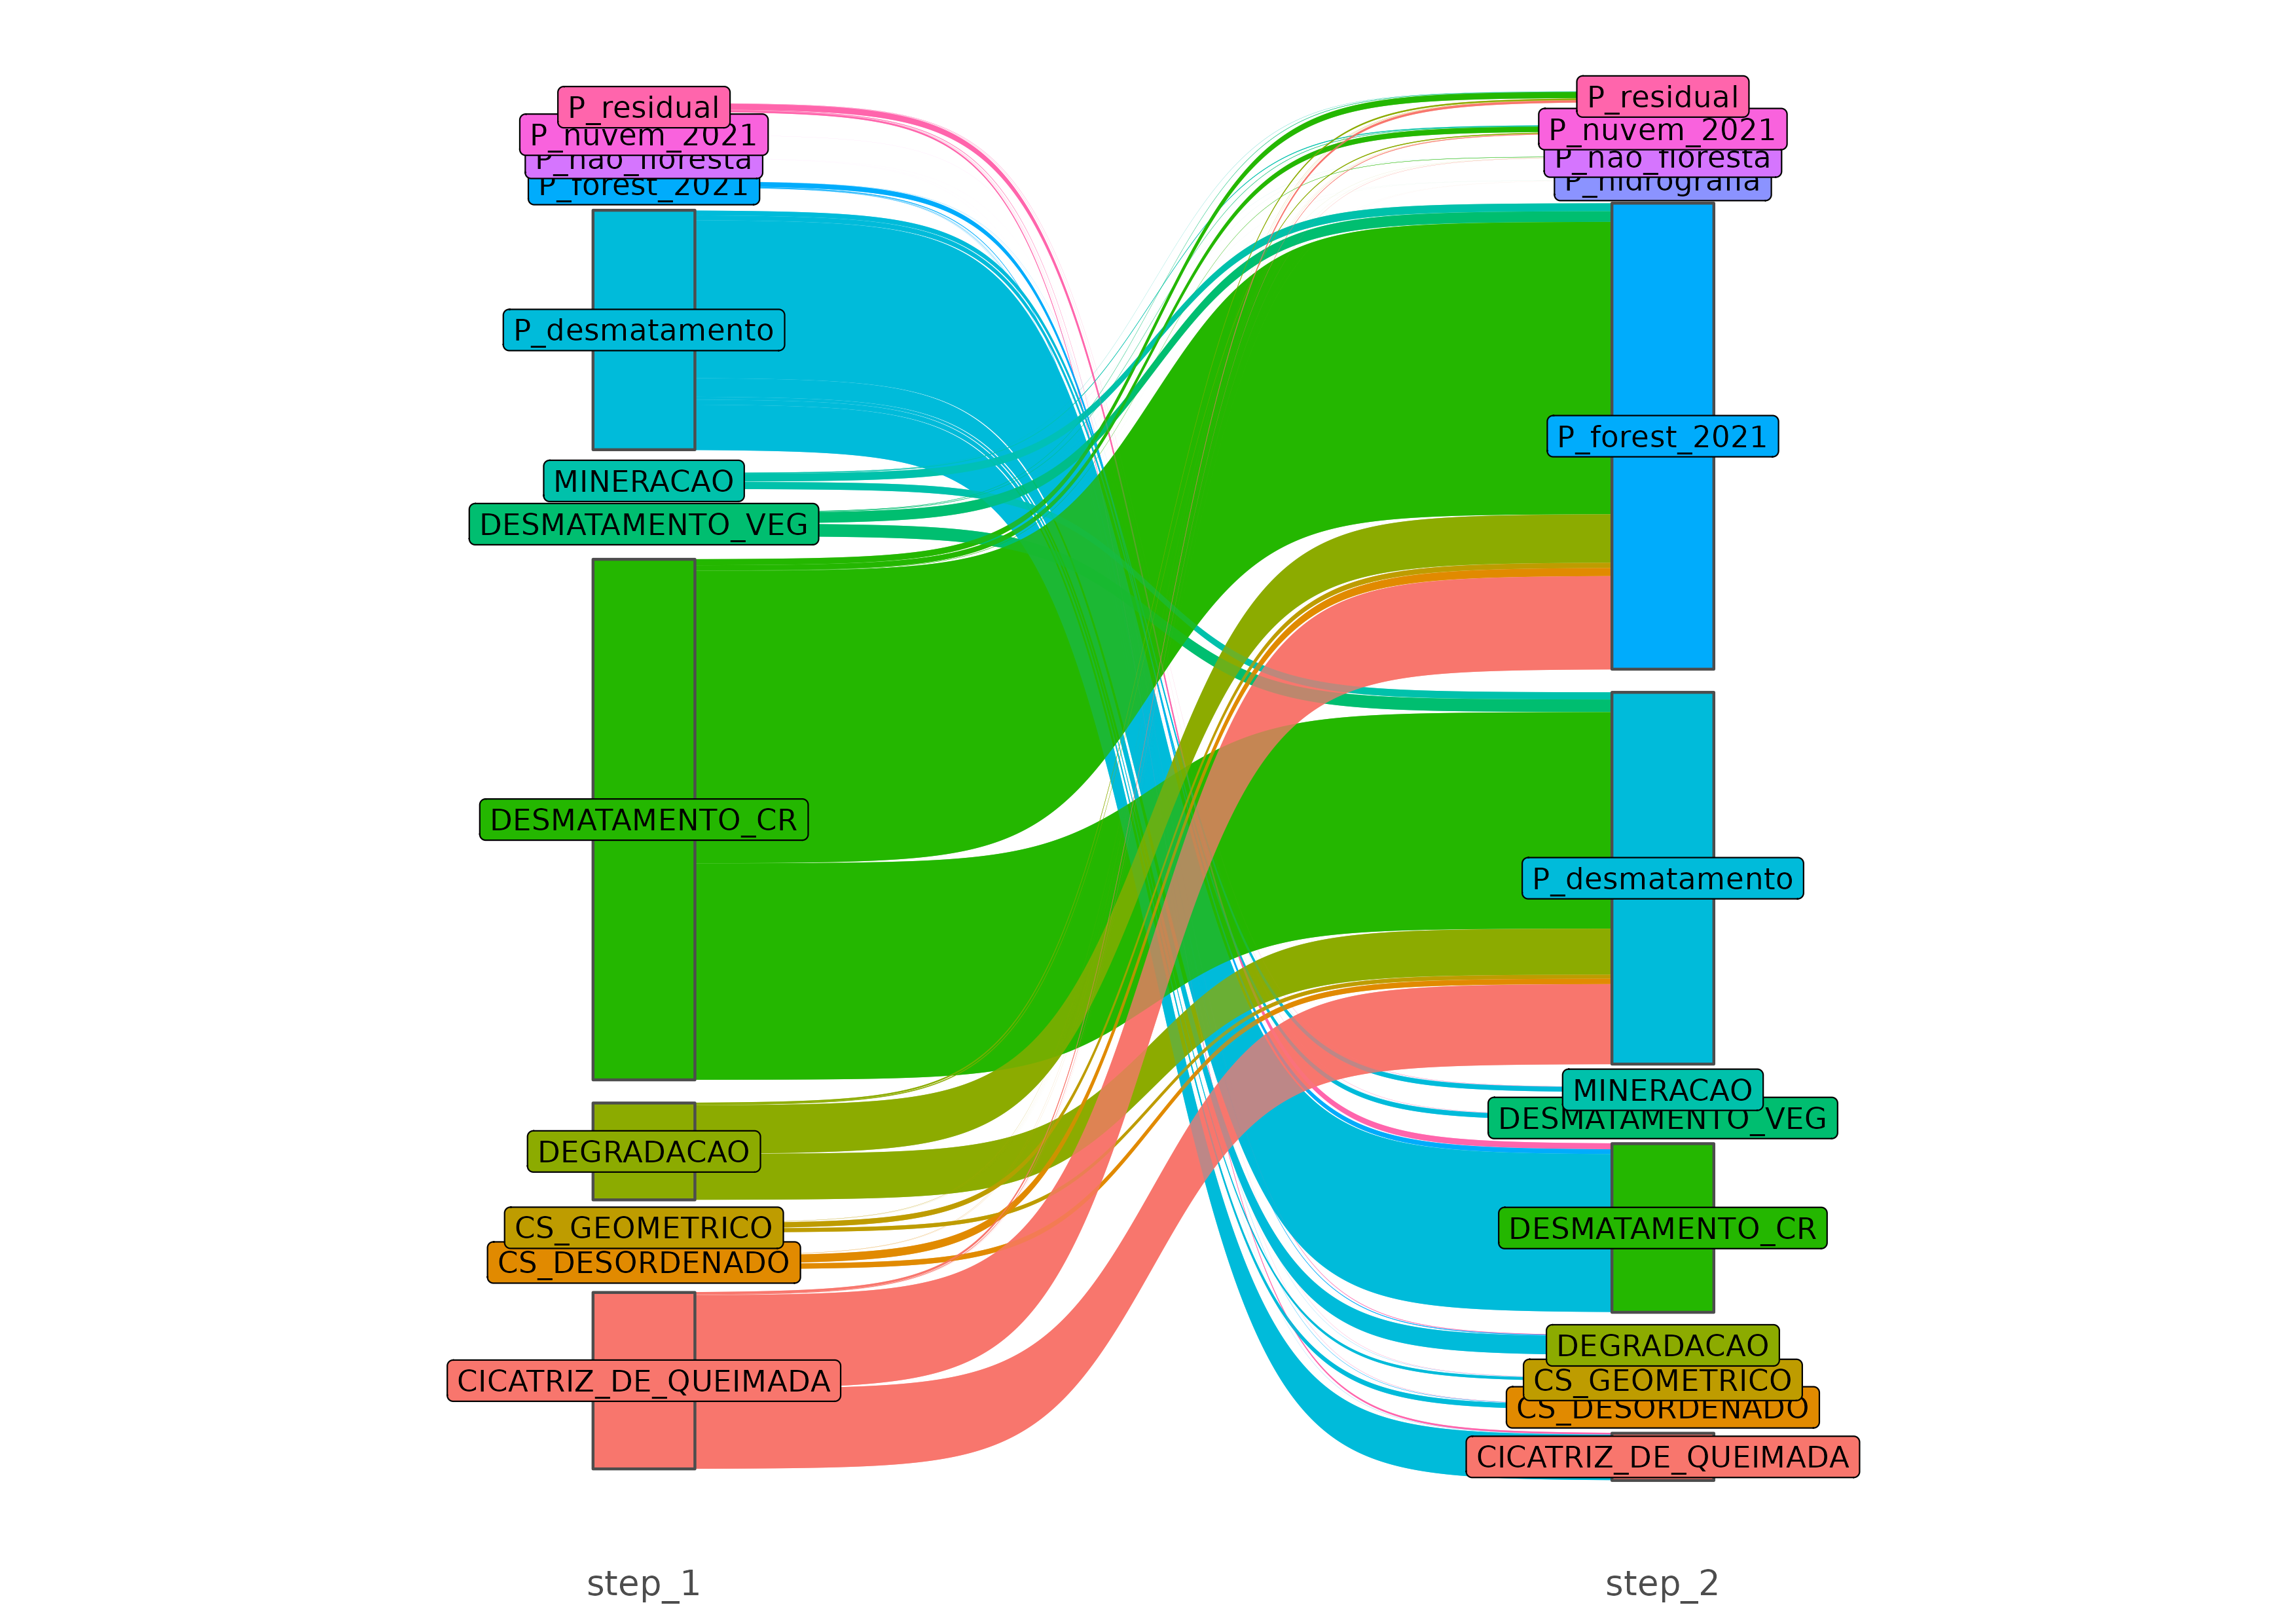
\includegraphics[width=0.65\linewidth]
        {./figures/plot_deter_prodes_subarea_trajectory_2.png}
        \caption{Tajectory of subareas with 2 wanings.}
        \label{fig:deter_prodes_subarea_trajectory_2}
    \end{figure}
\end{frame}

\begin{frame}
    \frametitle{DETER - PRODES subareas}
    \begin{figure}[h] 
        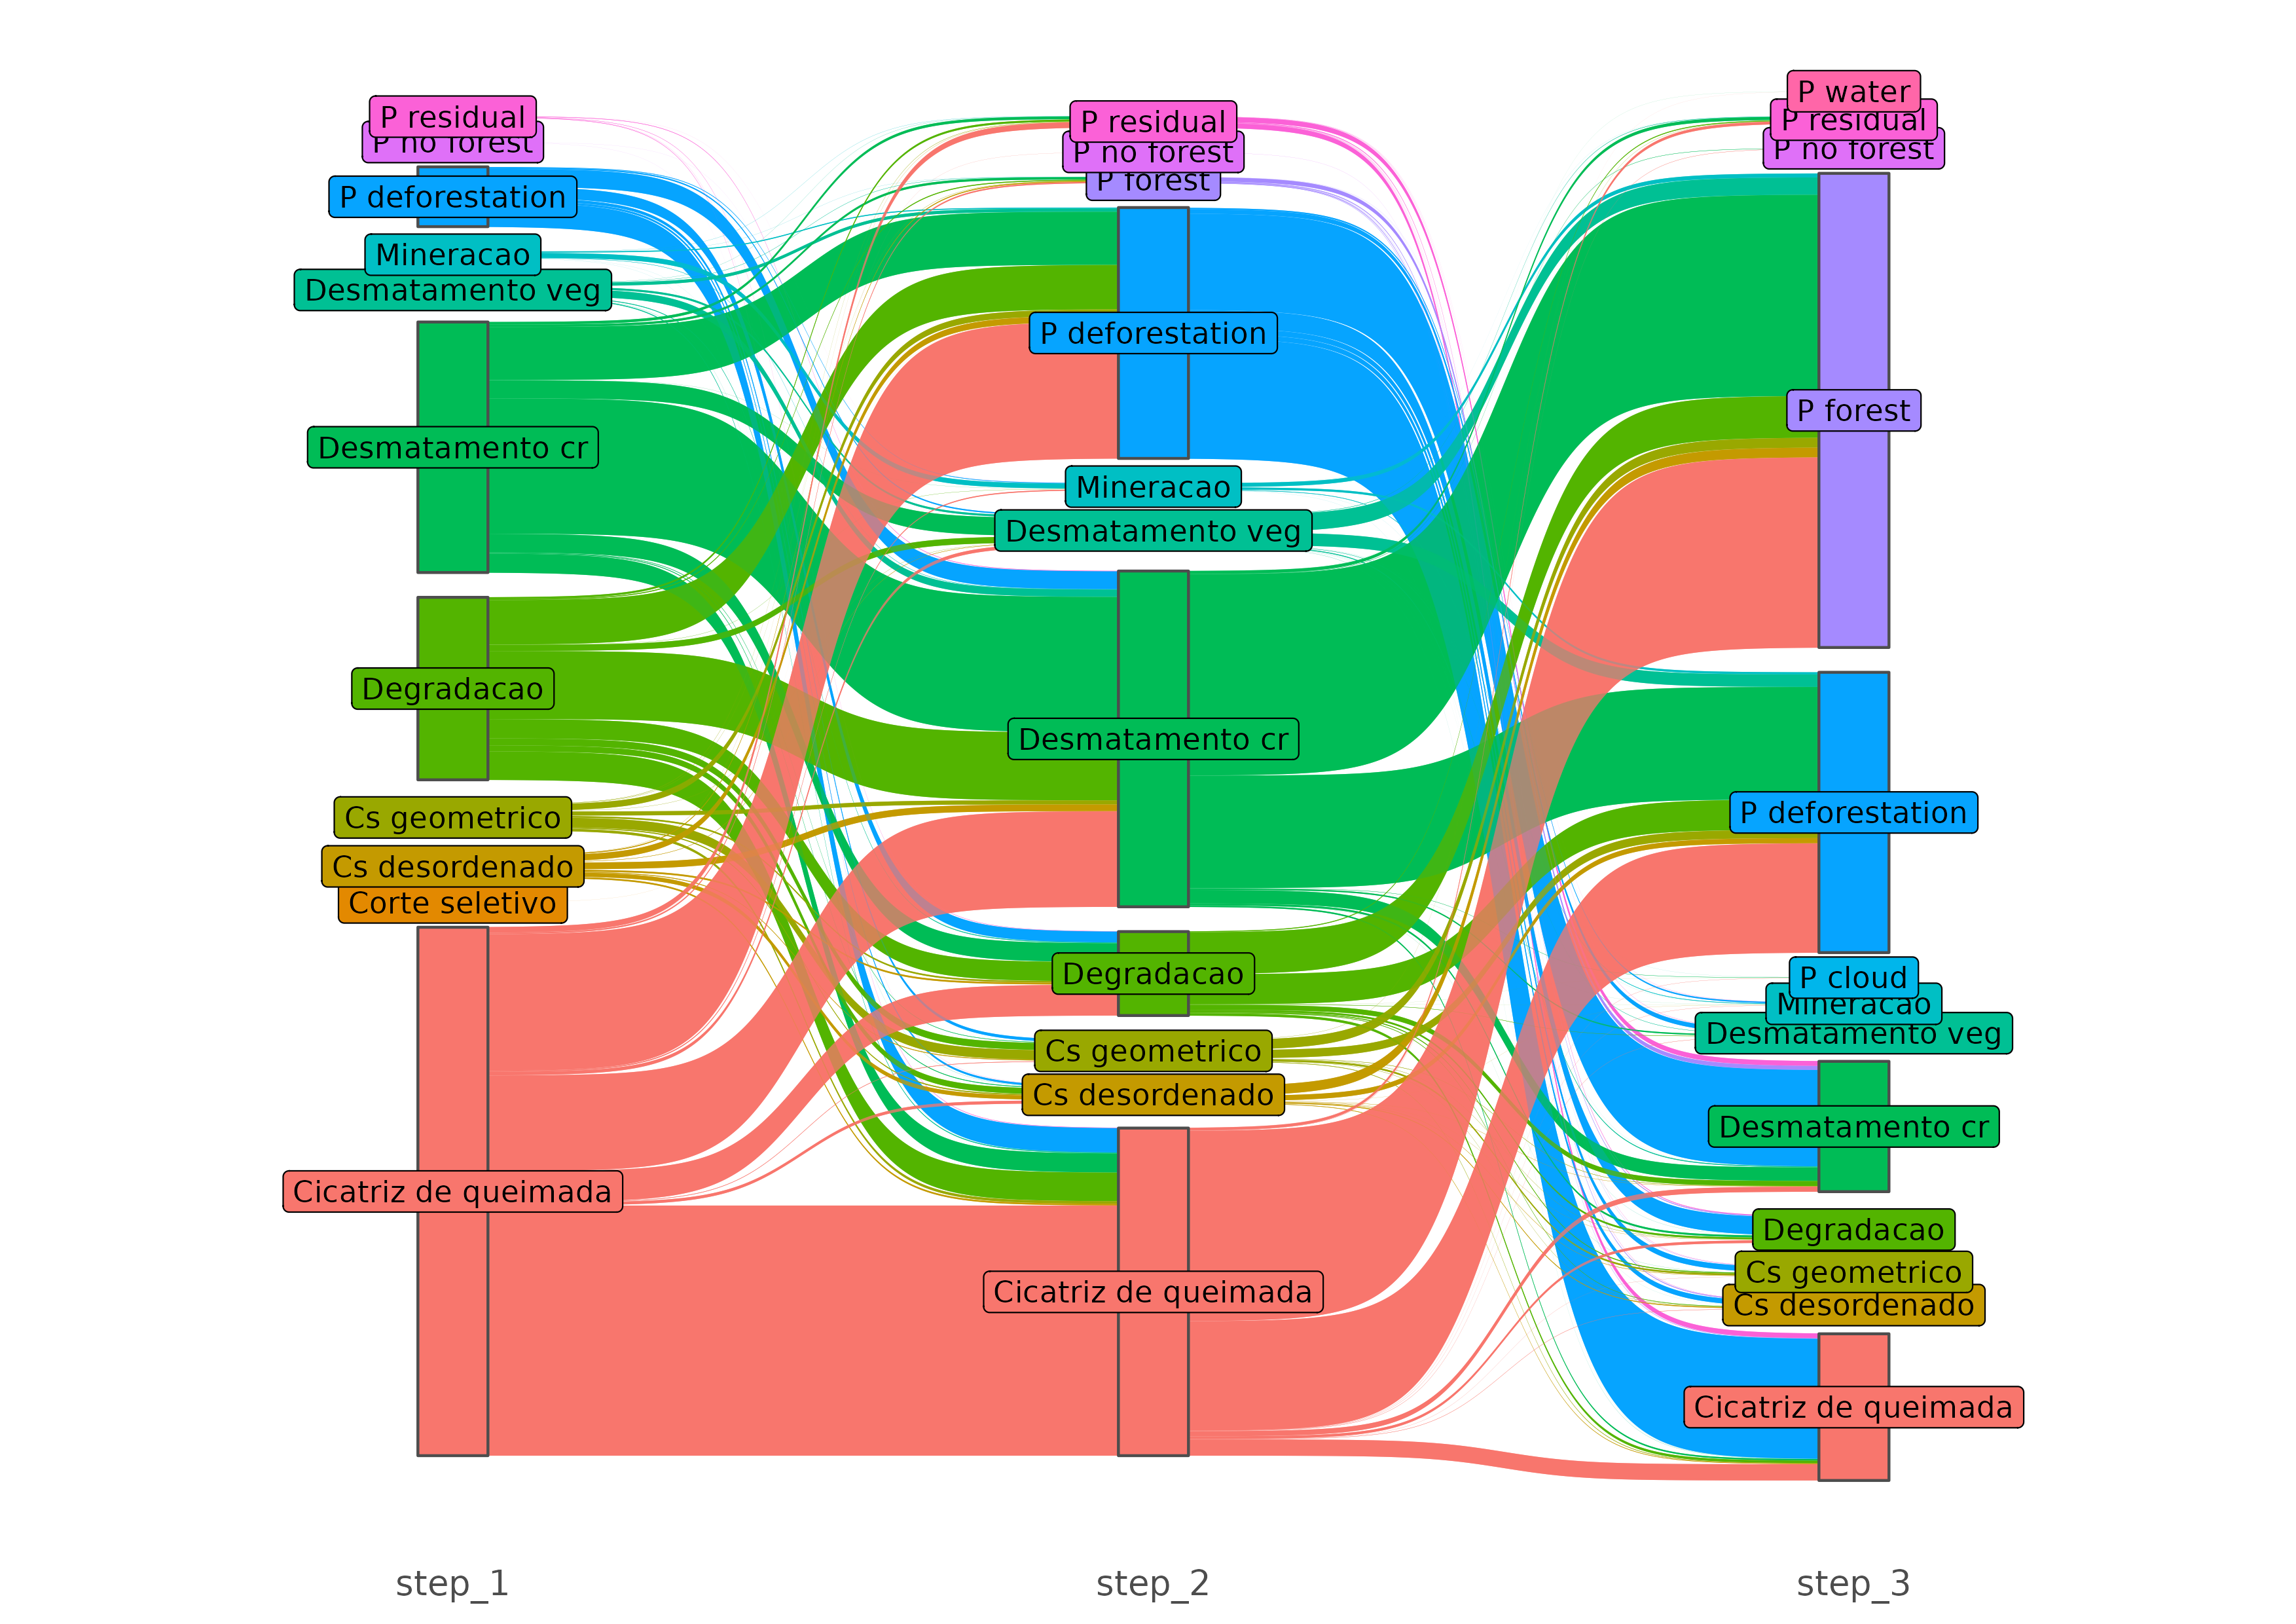
\includegraphics[width=0.65\linewidth]
        {./figures/plot_deter_prodes_subarea_trajectory_3.png}
        \caption{Tajectory of subareas with 3 wanings.}
        \label{fig:deter_prodes_subarea_trajectory_3}
    \end{figure}
\end{frame}

\begin{frame}
    \frametitle{DETER - PRODES subareas}
    \begin{figure}[h] 
        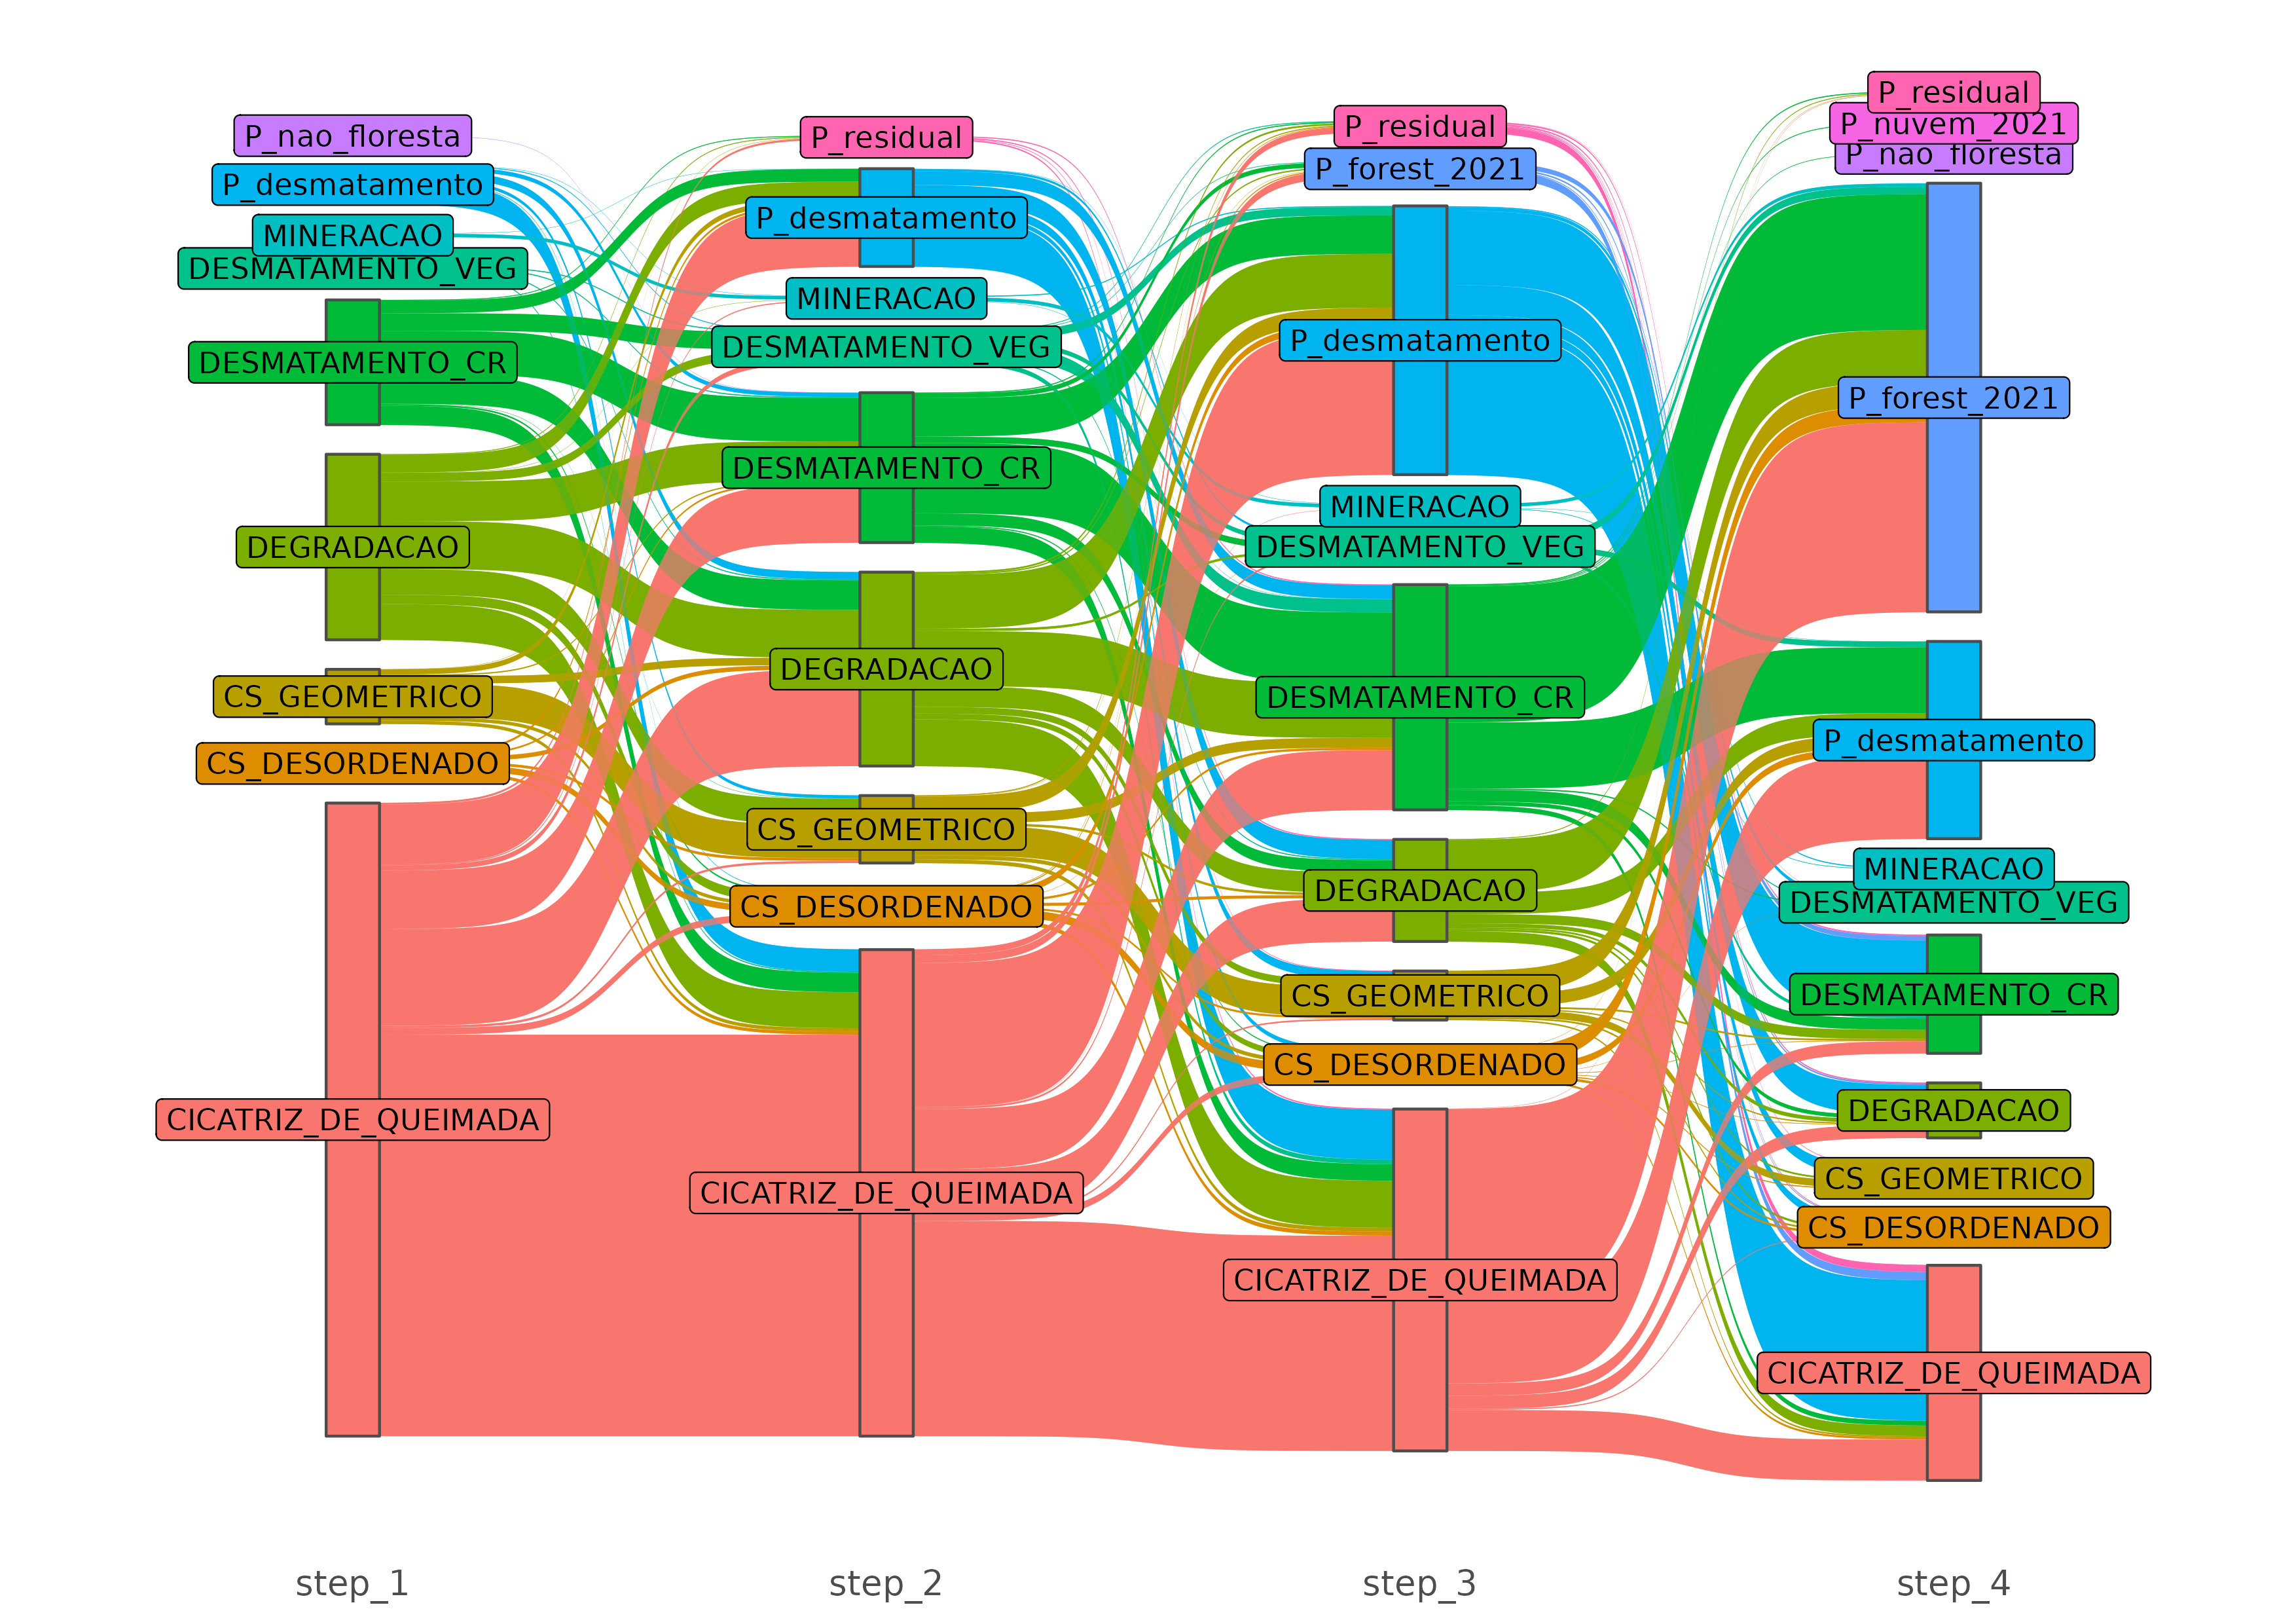
\includegraphics[width=0.65\linewidth]
        {./figures/plot_deter_prodes_subarea_trajectory_4.png}
        \caption{Tajectory of subareas with 4 wanings.}
        \label{fig:deter_prodes_subarea_trajectory_4}
    \end{figure}
\end{frame}


\begin{frame}
    \frametitle{DETER - PRODES subareas}
    \begin{figure}[h] 
        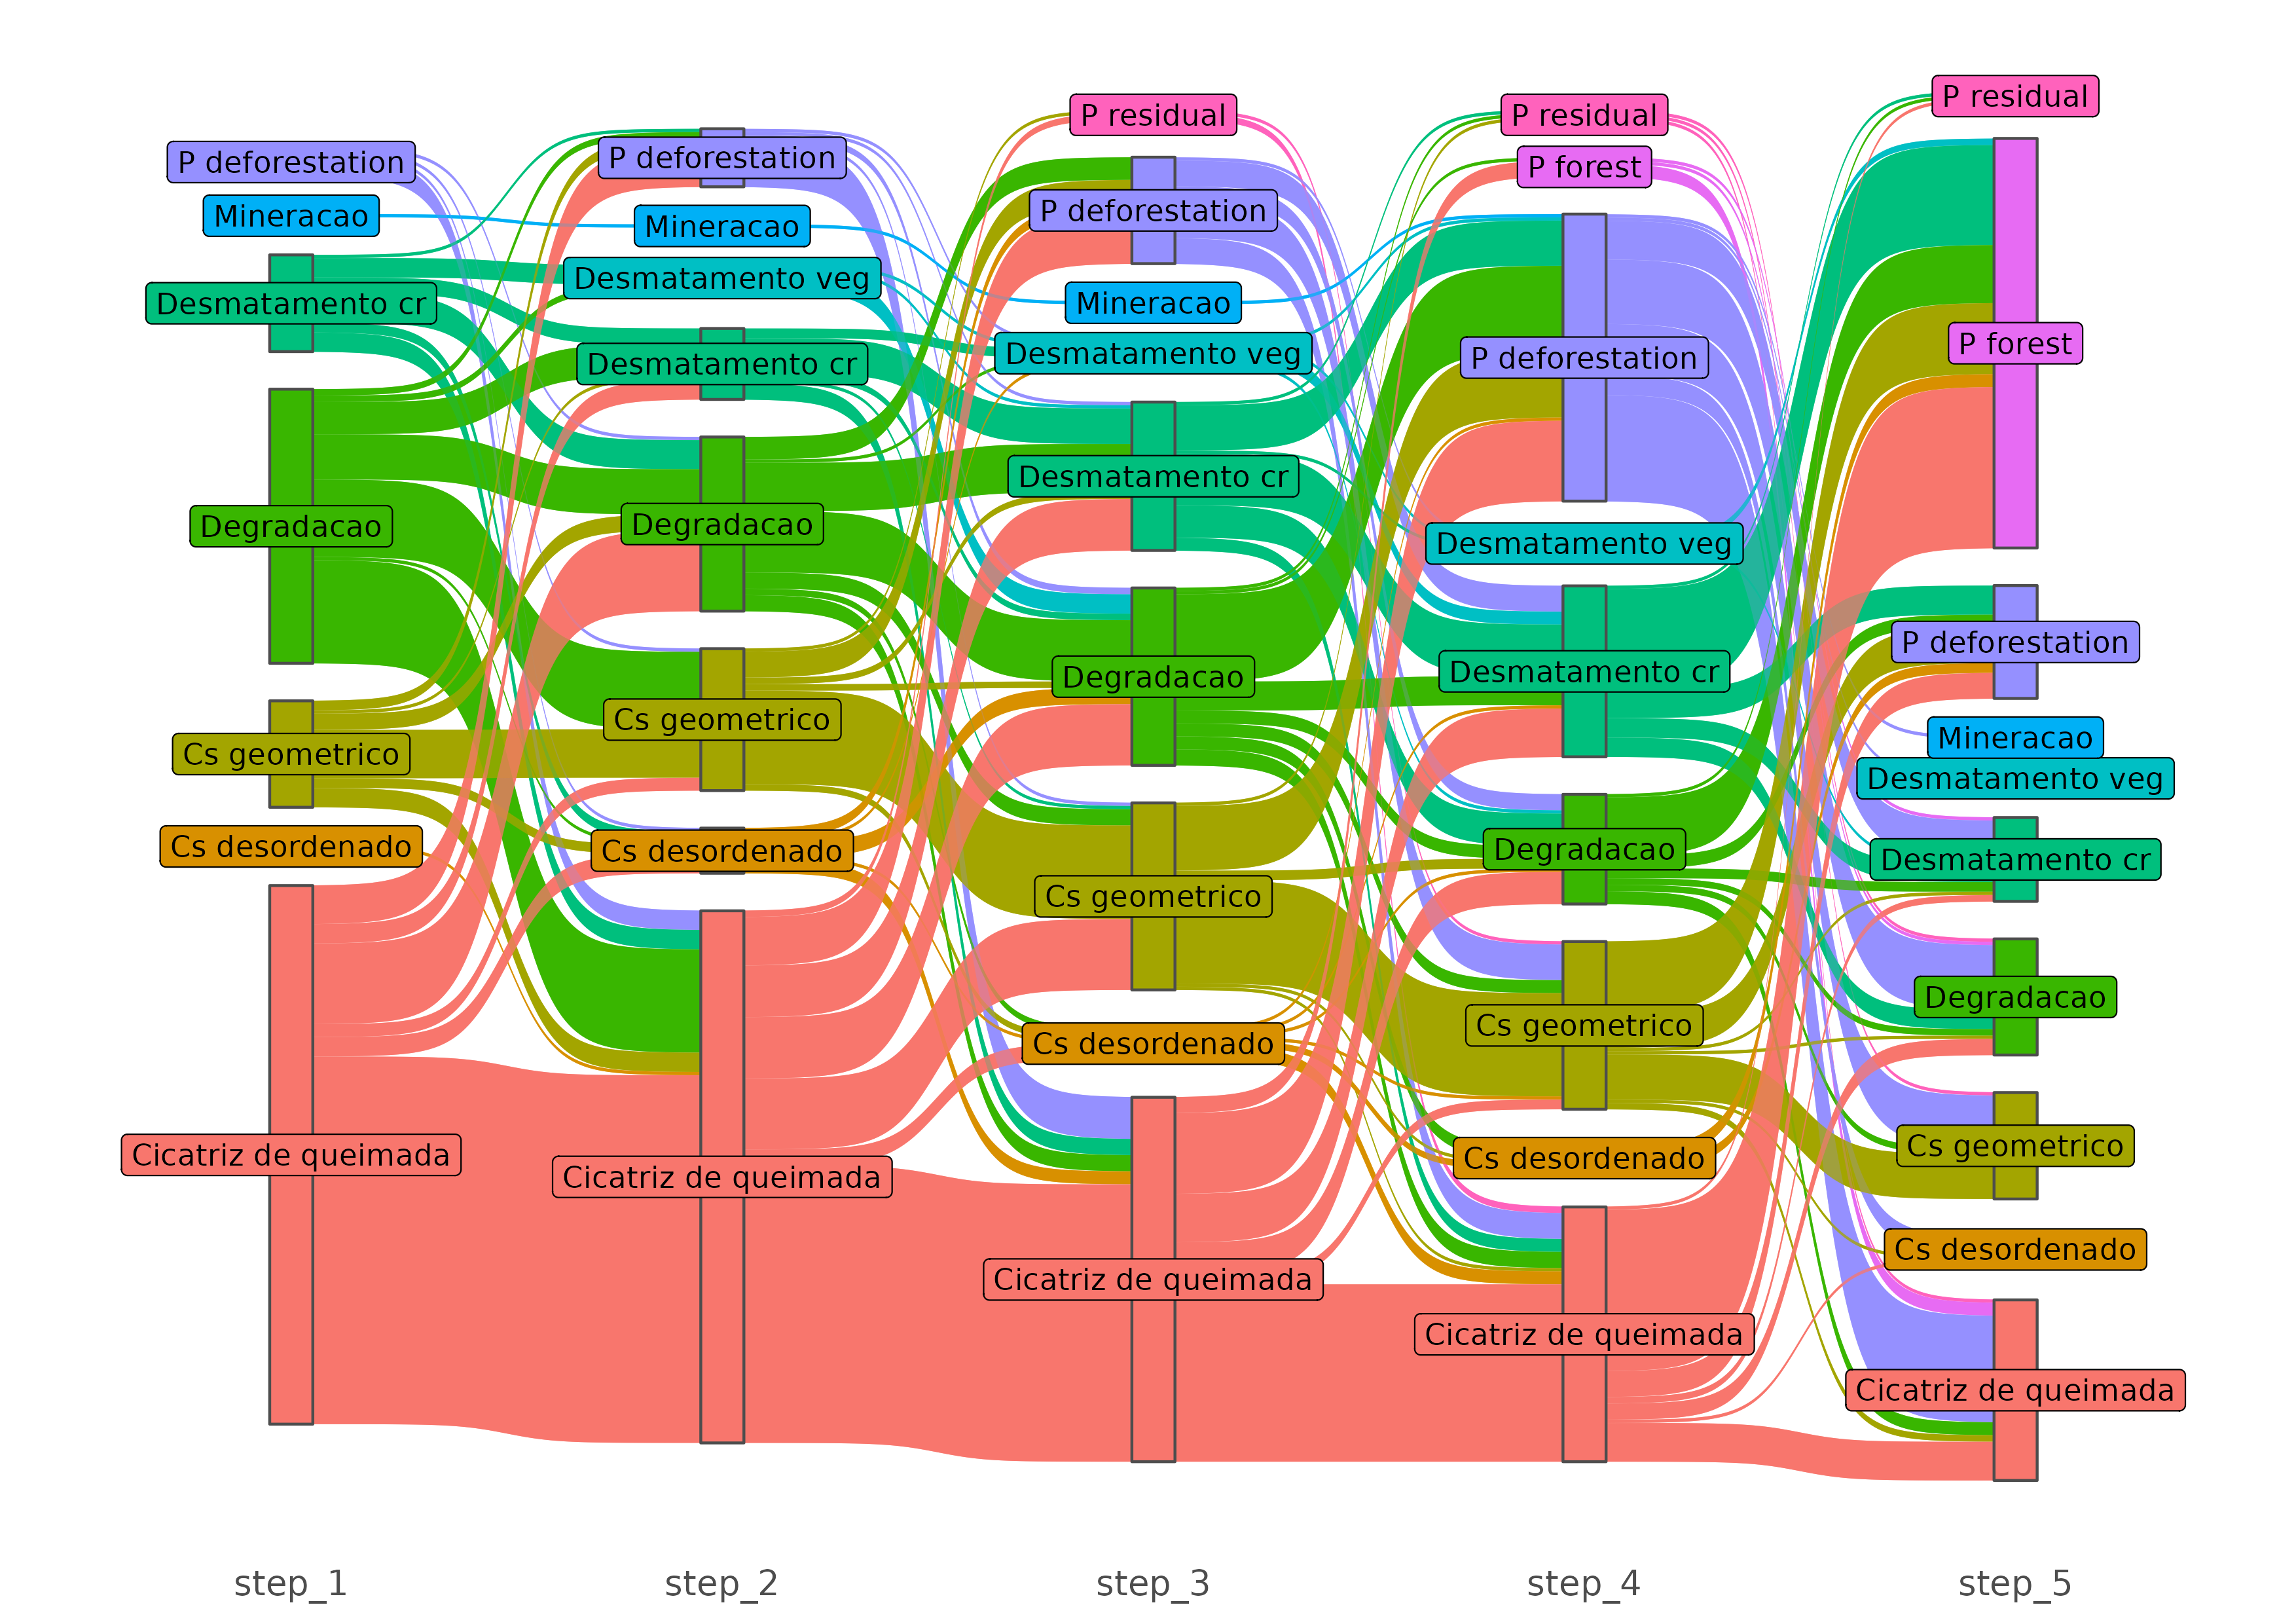
\includegraphics[width=0.65\linewidth]
        {./figures/plot_deter_prodes_subarea_trajectory_5.png}
        \caption{Tajectory of subareas with 5 wanings.}
        \label{fig:deter_prodes_subarea_trajectory_5}
    \end{figure}
\end{frame}

\begin{frame}
    \frametitle{DETER - PRODES subareas}
    \begin{figure}[h] 
        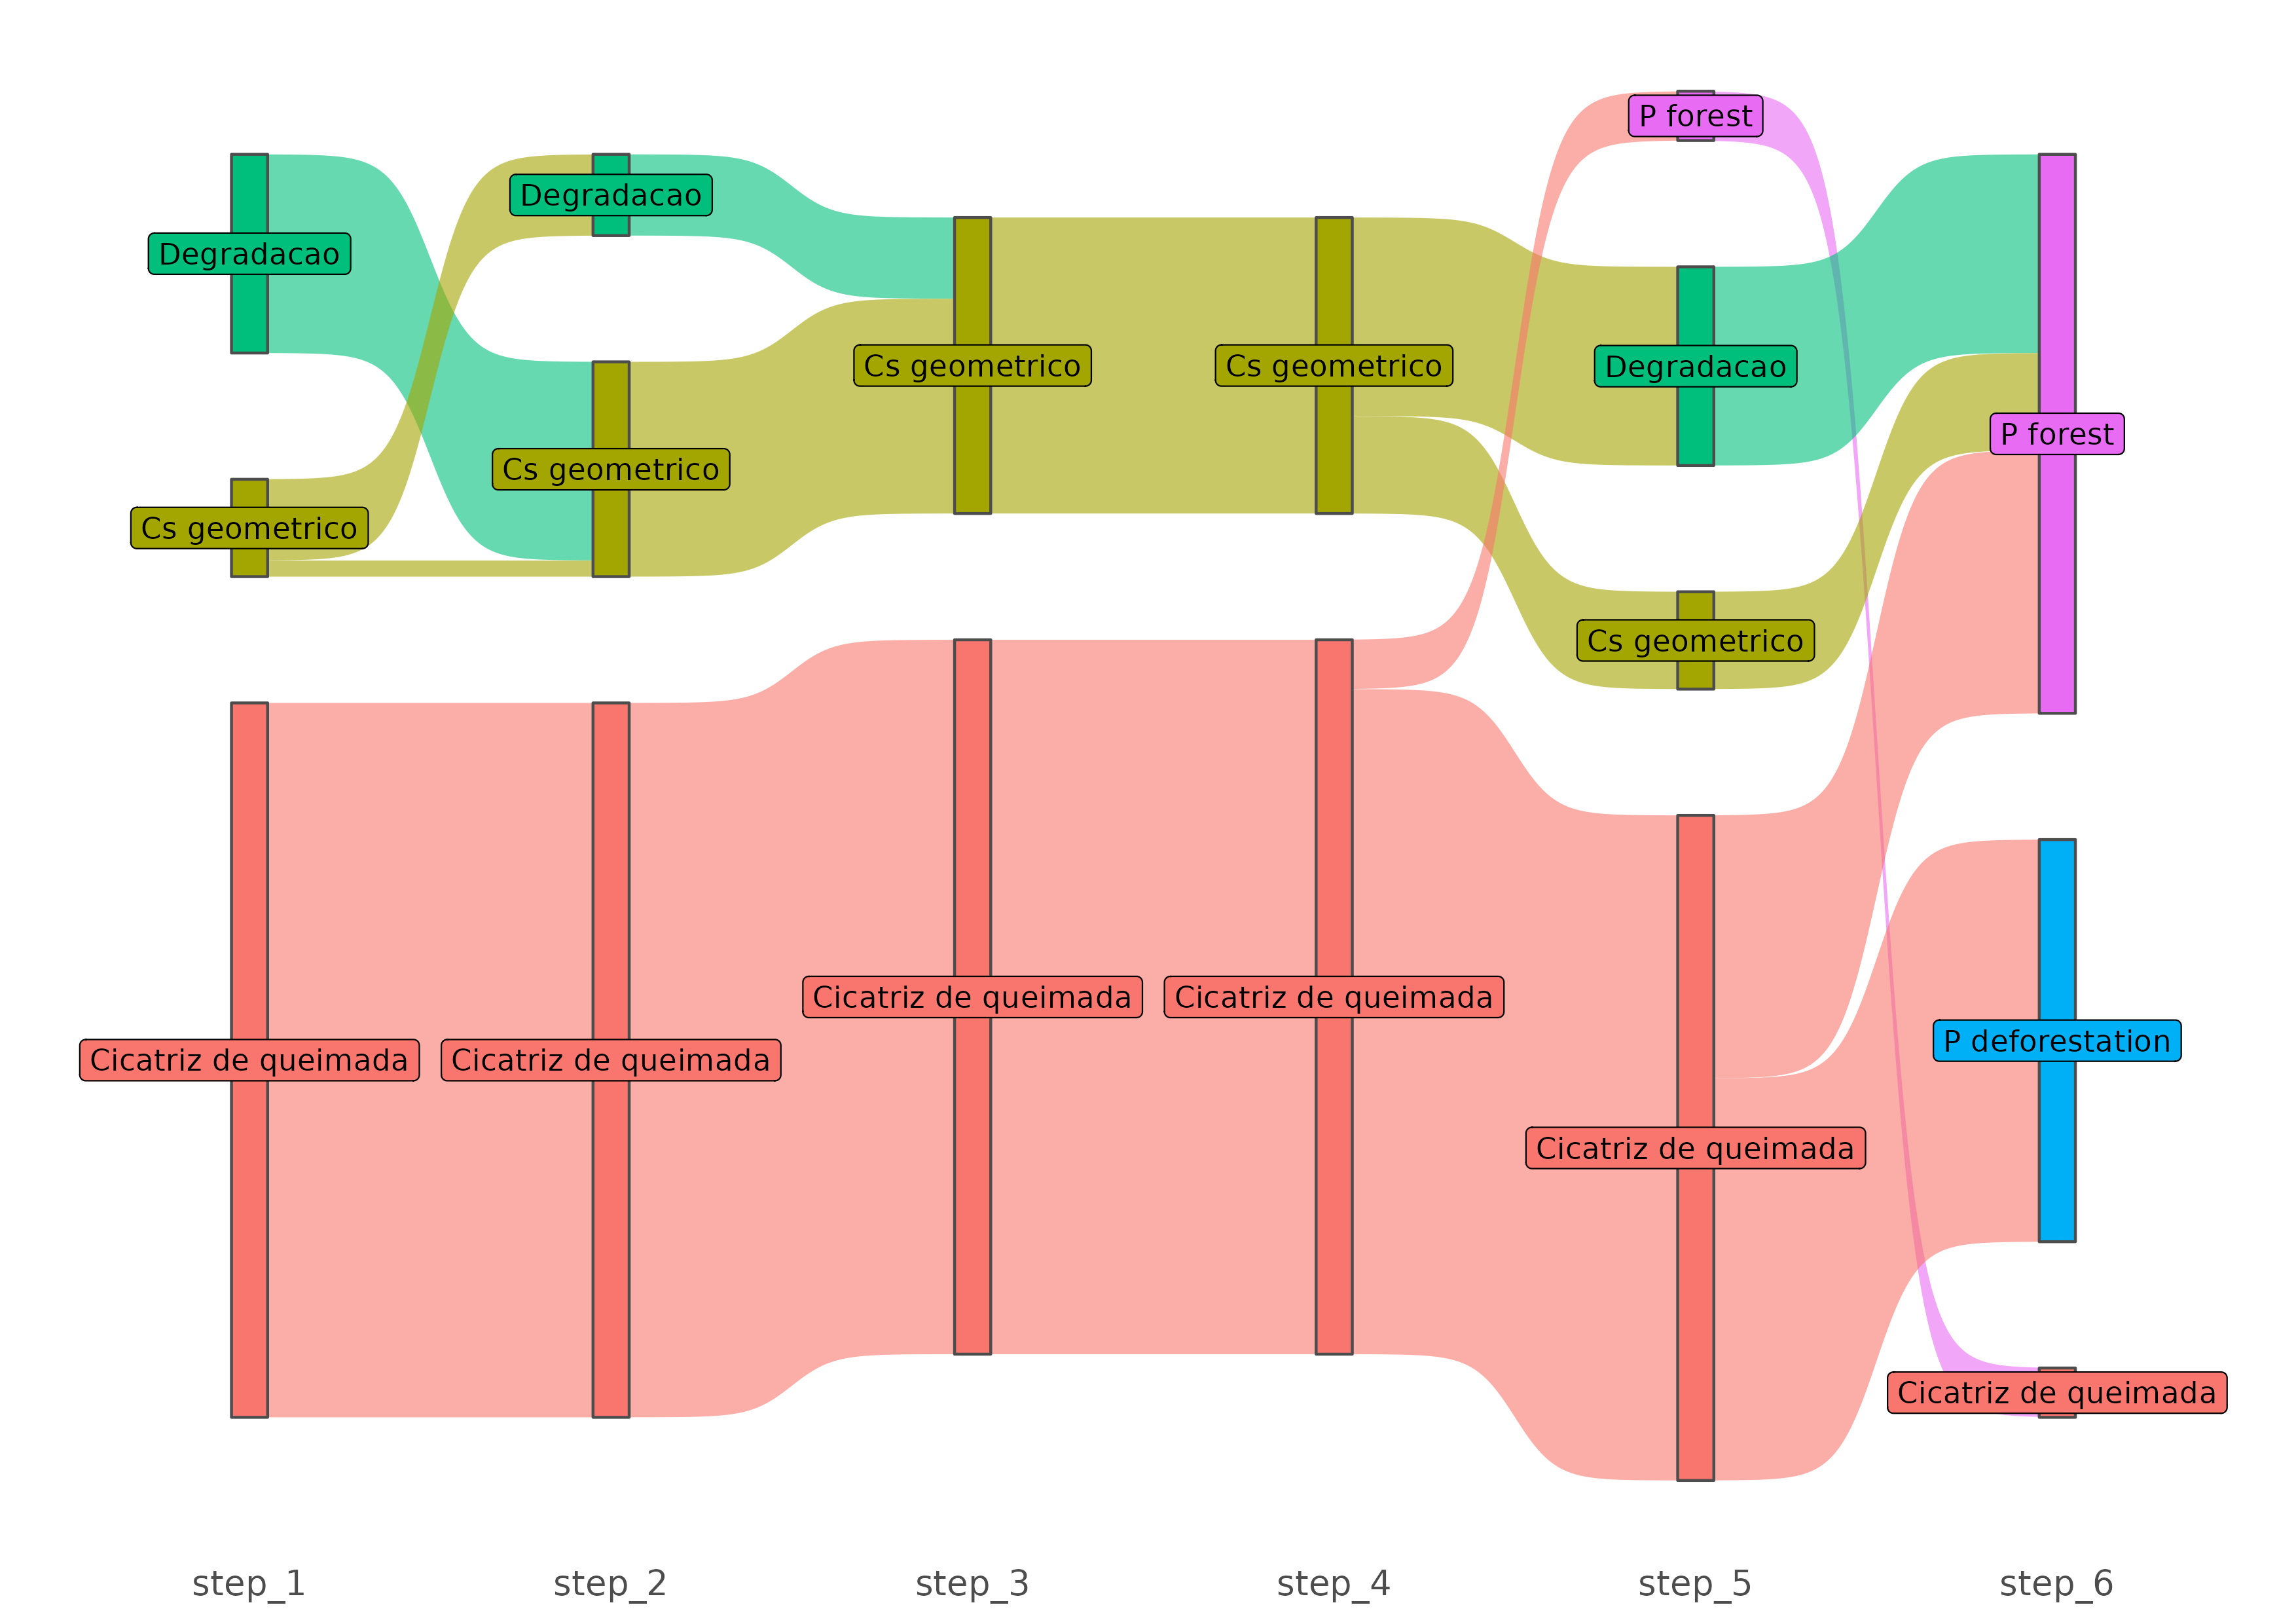
\includegraphics[width=0.65\linewidth]
        {./figures/plot_deter_prodes_subarea_trajectory_6.png}
        \caption{Tajectory of subareas with 6 wanings.}
        \label{fig:deter_prodes_subarea_trajectory_6}
    \end{figure}
\end{frame}


%---- Closing ----

\begin{frame}
    \frametitle{Final remarks}
    \begin{itemize}
        \item The analysis of DETER warning subareas along time could improve 
            the characterization of forest degradation along time.
        \item Potential applications of our work are:
            \begin{itemize}
                \item Improve estimation of emissions of greenhouse gases, i.e.
                    our data could help avoiding double counting.
                \item Identify spatio-temporal areas which could help training 
                    Machine-Learning algorithms for automatic indentification 
                    of forest degradation.
            \end{itemize}
        \item Code available at 
            \url{https://github.com/albhasan/treesburnareas}
    \end{itemize}
\end{frame}

\begin{frame}[allowframebreaks]
    \frametitle{References}
    \bibliographystyle{amsalpha}
    \bibliography{07_SBSR.bib}
\end{frame}

\end{document}
